\documentclass[11pt,a4paper]{article}
\usepackage[T1]{fontenc}
\usepackage[utf8]{inputenc}
\usepackage{authblk}
\usepackage[english]{babel}
\usepackage{fancyhdr}
\usepackage{subfig}
\usepackage{floatrow}
\usepackage{float}
\usepackage{amsmath}
\usepackage{amssymb}
\usepackage{slashed}
\usepackage{graphicx}
\usepackage{todonotes}
\usepackage[toc,page]{appendix}
\usepackage{hyperref}
\usepackage{placeins}
\usepackage{cleveref}
\usepackage{multirow}
\usepackage{longtable}
\usepackage[final]{pdfpages}
\usepackage[export]{adjustbox}
\usepackage[final]{pdfpages}
\hypersetup{
	colorlinks,
	citecolor=purple,
	filecolor=black,
	linkcolor=blue,
	urlcolor=black
}
\usepackage{color}

\newcommand{\white}[1]{{\textcolor{white}{#1}}}



\newcommand*\samethanks[1][\value{footnote}]{\footnotemark[#1]}
%\title{Transition Form Factor of the $\eta^{\prime}$ Meson with CLAS12}
\title{Measurement of Cross-Sections of exclusive $\pi^{0}$ Photo-production on Hydrogen from 1.1 GeV - 5.45 GeV using $\lowercase{e}^{+}\lowercase{e}^{-}\gamma$ decay from the CLAS/g12 Data}
\date{}

\author{Michael C. Kunkel\thanks{email: m.kunkel@fz-juelich.de}\thanks{Now at Forschungszentrum J\"ulich, J\"ulich (Germany)} \\ \vspace{0.3cm} \it \qquad Old Dominion University, VA (U.S.A.) \newline \newline}


\renewcommand\Authands{, }
\fancypagestyle{firststyle}
{
	\fancyhf{}
	\renewcommand{\headrulewidth}{0pt}
	\fancyhead[R]{\small CLAS ANALYSIS XXX}
}
\newlength{\figwidth}
\setlength{\figwidth}{0.9\columnwidth}

\newlength{\qfigheight}
\setlength{\qfigheight}{0.25\textheight}

\newlength{\hfigheight}
\setlength{\hfigheight}{0.5\textheight}

\def\piz{\pi^{0}}
\def\pizT{$\pi^{0} \ $}
\def\pizDal{$\pi^{0} \rightarrow e^+e^- \gamma  $}

\def\etaT{$\eta $}
\def\etaDal{$\eta \rightarrow e^+e^- \gamma  $}

\def\omT{$\omega  $}
\def\omDal{$\omega \rightarrow e^+e^- \piz $}

\def\etaP{\eta^{\prime}}
\def\etaTP{$\eta^{\prime}  $}
\def\etaPDal{$\eta^{\prime} \rightarrow e^+e^- \gamma  $}

\def\phiT{$\phi  $}
\def\phiDal{$\phi \rightarrow e^+e^- \eta  $}
\def\phiDalT{\phi \rightarrow e^+e^- \eta  }

\def\epemT{$ e^+e^-  $}
\def\epem{e^+e^-}
\def\pipiT{$\pi^+\pi^-$}
\def\pipi{\pi^+\pi^-}


\def\phiPR{$ep\to e'p \phi \rightarrow p e^+e^- \eta$}
\def\etaPR{$ep\to e'p \etaP \rightarrow p e^+e^- \gamma$}

%\def\grpath{figures}
%\def\figures{/Users/michaelkunkel/WORK/GIT_HUB/THESIS/figures/print}
\def\figures{/Volumes/Mac_Storage/Work_Codes/GIT_HUB/THESIS/figures/print}

\newcommand{\abbr}[1]{\textsc{\texttt{#1}}}
\newcommand{\abbrlc}[2]{\textsc{\texttt{#1}}\texttt{#2}}
%%%% new commands and macros %%%%%%%%%%%%%%%%%%%%%%%%%%%%%%%%%%%%%%%%%%%
\newlength{\figwidth}
\setlength{\figwidth}{0.9\columnwidth}

\newlength{\qfigheight}
\setlength{\qfigheight}{0.25\textheight}

\newlength{\hfigheight}
\setlength{\hfigheight}{0.5\textheight}

\newcommand{\dedicationfont}{\fontencoding{T1}\fontfamily{anttlc}\fontseries{m}\fontshape{n}\fontsize{12}{15}\selectfont}

\newcommand{\acro}[1]{#1\@}
\newcommand{\abbr}[1]{\textsc{\texttt{#1}}}
\newcommand{\abbrlc}[2]{\textsc{\texttt{#1}}\texttt{#2}}
\newcommand{\desg}[1]{\texttt{#1}}
\newcommand{\todo}[1]{\textbf{\uppercase{\emph{#1}}}} %\textcolor{Orange}{#1}}}


%Some variables
%
%
\def\g12{\emph{g12}}

\def\G11{\emph{g11}}
\def\clas{\abbr{CLAS }}

\def\Lqcd{\mathcal{L}_{\mathtt{QCD}}}
\def\qfield{\psi}
\def\qbarfield{\overline{\psi}}

\def\grpath{/Users/michaelkunkel/WORK/GIT_HUB/THESIS/figures/print}
\def\figures{/Users/michaelkunkel/WORK/GIT_HUB/THESIS/figures/print}
\def\tablepath{../../}
\newcommand{\bank}[4]{$\mathtt{#1}^{#2}_{#3}\lbrack\mathtt{#4}\rbrack$}

\def\ith{$i$\textsuperscript{th}}

\def\um{{\text{$\mu$}}m}

%\def\coloronline{(Color online.)\ }
\def\coloronline{}

%%% particles
\def\p{\mathrm{p}}
\def\n{\mathrm{n}}
\def\Kp{\mathrm{K}^{+}}
\def\Km{\mathrm{K}^{-}}
\def\K0{\mathrm{K}^{0}}
\def\Y{\mathrm{Y}}
\def\epos{\mathrm{e}^{+}}
\def\eneg{\mathrm{e}^{-}}
\def\gamstar{\mathrm{$\gamma$}^{*}}
\def\piup{$\pi$}
\def\gammaup{$\gamma$}
%%% TAGGER and RF related times
\def\trf{t_{\mathtt{RF}}}
\def\ttag{t_{\mathtt{TAG}}}
\def\ttagrf{t_{\mathtt{TAG,RF}}}
\def\tprop{t_\mathrm{prop}}
\def\ttrigoffset{t_{\mathrm{trigger-offset}}}

%%% BEAM energy
\def\ebeam{E_{\mathrm{beam}}}

%%% Beta
\def\betasttof{\beta_{\mathtt{ST-TOF}}}
\def\betatof{\beta_{\mathrm{vtx}\mathtt{-TOF}}}
\def\betap{\beta_{p}}

%%% path lengths
\def\lst{\ell_{\mathtt{ST}}}
\def\ltof{\ell_{\mathtt{TOF}}}
\def\lsttof{\ell_{\mathtt{ST-TOF}}}

%%% raw subsystem times
\def\tst{t_{\mathtt{ST}}}
\def\ttof{t_{\mathtt{TOF}}}
\def\dtsttof{\Delta t_{\mathrm{ST-TOF}}}

%%% vertex times
\def\tv{t_{\mathrm{vtx}}}
\def\tvtagrf{t_{\mathrm{vtx}}(\mathtt{TAG_{RF}})}
\def\tvst{t_{\mathrm{vtx}}(\mathtt{ST})}

\def\adcst{\mathtt{ADC}_{\mathtt{ST}}}

\newcommand{\bra}[1]{\left<#1\right|}
\newcommand{\ket}[1]{\left|#1\right>}
\newcommand{\braket}[2]{\left<#1\middle|#2\right>}
\def\piz{$\mathrm{\pi^{0}}\ $}
\def\epem{$e^+e^-\ $}
% Document starts
\begin{document}
	\setcounter{page}{3}
%	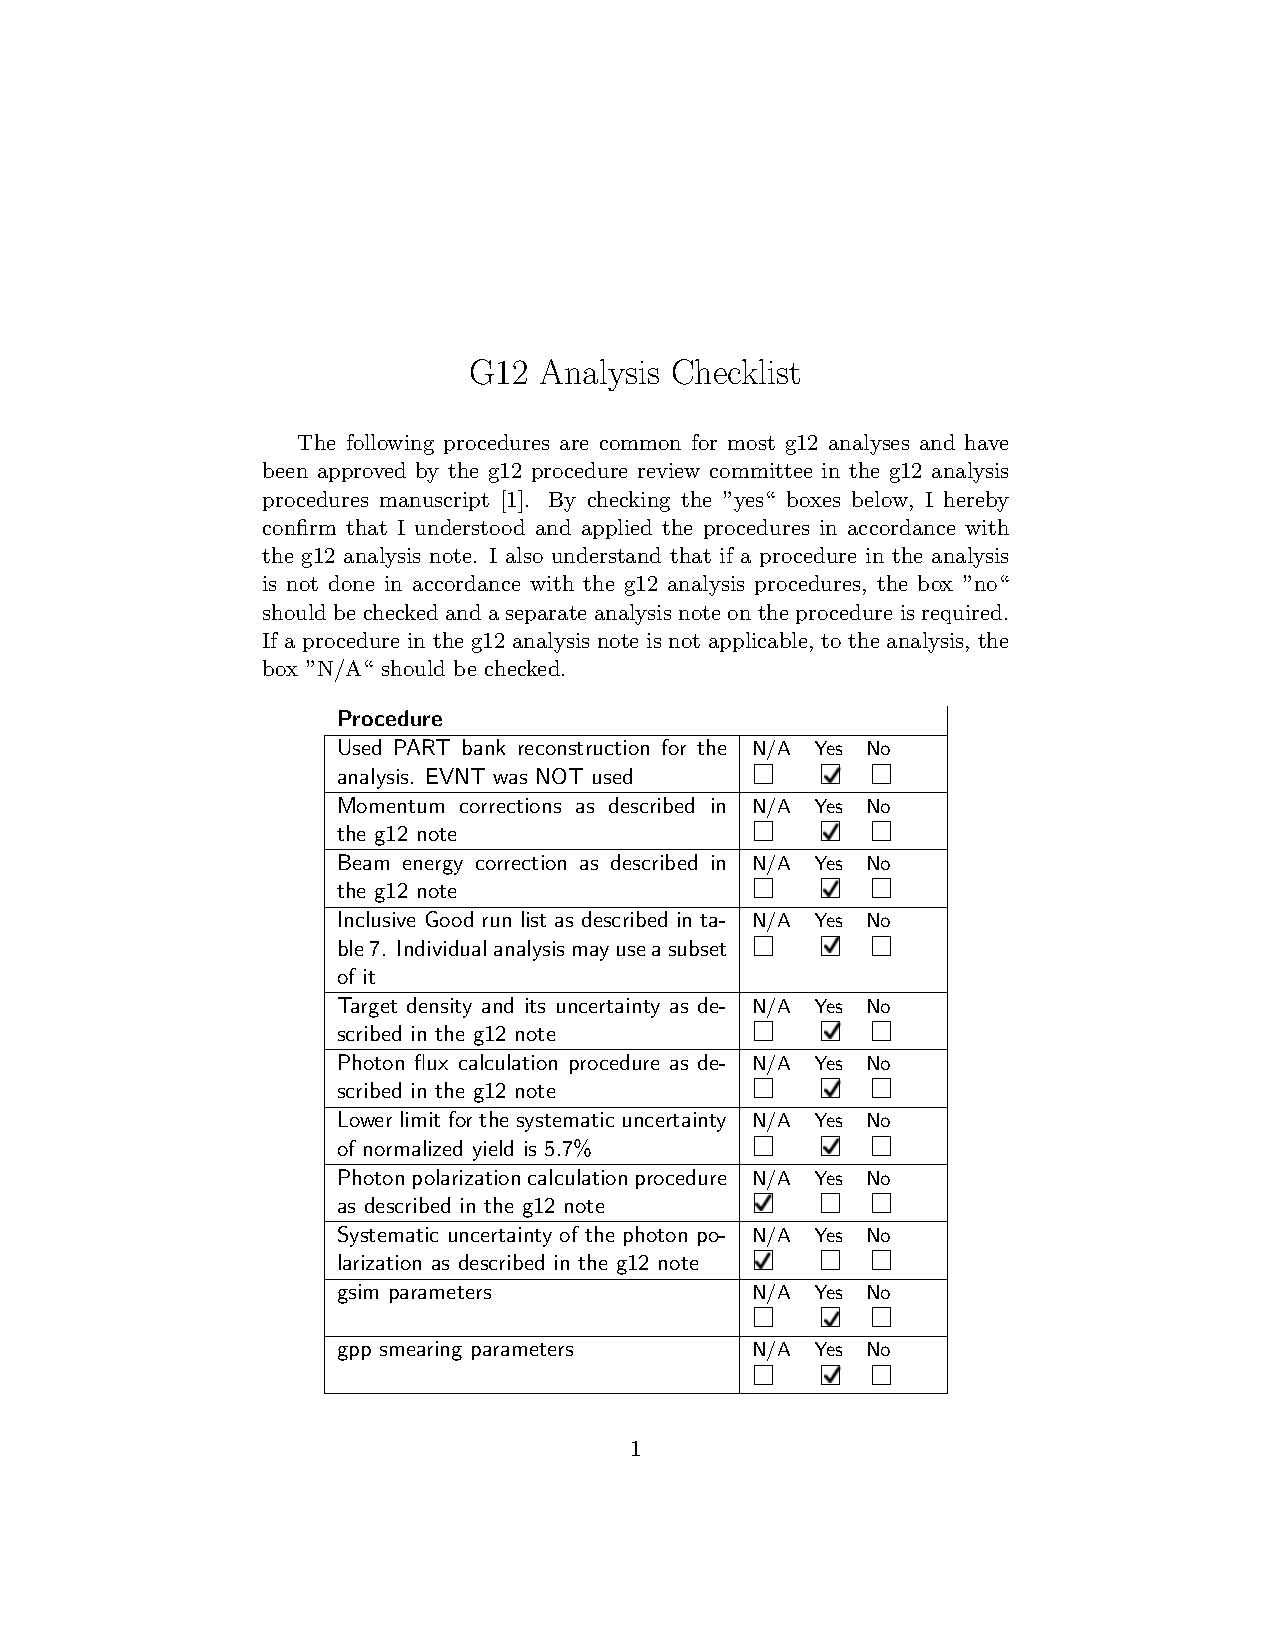
\includepdf[pages=-]{CheckList_II_final.pdf}
	\maketitle
	\thispagestyle{firststyle}
\begin{abstract}
	Photoproduction of the $\pi^0$ meson was studied using the \textsc{\texttt{CLAS}} detector at Thomas Jefferson National Accelerator Facility using tagged incident beam energies spanning the range $E_{\gamma}=$~1.1~GeV~-~5.45~GeV. The measurement is performed on a liquid hydrogen target in the reaction $\gamma p\to pe^+e^-(\gamma)$. The final state of the reaction is the sum of two subprocesses for $\pi^0$ decay, the Dalitz decay mode of $\pi^0\to e^+e^-\gamma$ and conversion mode where one photon from $\pi^0\to \gamma\gamma$ decay is converted into a $e^+e^-$ pair. This specific final state reaction avoided limitations caused by single prompt track triggering and allowed a kinematic range extension to the world data on $\pi^0$ photoproduction to a domain never systematically measured before.
	
	We report the measurement of the $\pi^0$ differential cross-sections $\frac{d\sigma}{d\Omega}$ and $\frac{d\sigma}{dt}$. The angular distributions agree well with the SAID parametrization for incident beam energies below 3~GeV, while an interpretation of the data for incident beam energies greater than 3~GeV is currently being developed.
\end{abstract}
	\newpage
	\tableofcontents
	\newpage
	\section{\label{sec:level1}Introduction}
In hadron physics, photoproduction of single pion is essential to understand the photon-nucleon vertex. At low energies, the photon-nucleon coupling establishes excited nucleon resonances which has been at the forefront of physics ''missing resonances'' search. At high energies single pion photoproduction can be used to test predictions of Regge theory, in which recent calculations~\cite{JPAC} have shown to describe the presented data well. Furthermore, these measurements have shown that the differential cross section for single pion photoproduction at fixed c.m. angles, $\theta_{c.m.}$, of $70^{\circ}$, $90^{\circ}$ and $110^{\circ}$ seem to scale as $\frac{d\sigma}{dt} \sim s^{2-n}f(\theta_{c.m.})$, where $s$ and $t$ are the Mandelstam variables and $n$ is the total number of interacting elementary fields in the initial and final state of the reaction. This is predicted by the constituent counting rule~\cite{scaling1,scaling2} and exclusive measurements in $pp$ and  $\bar{p}p$ elastic scattering~\cite{scalingexp5, scalingexp7}, meson-baryon $M p$ reactions~\cite{scalingexp7}, and photoproduction $\gamma N$~\cite{scalingexp2, scalingexp3, scalingexp4, scalingexp6, scalingexp8, scalingexp9, scalingexp10, scalingexp11} agree well with this rule. The following paper details the CLAS g12 experiment, the extraction of single neutral pion photoproduction from data, the differential cross-sections through the entire beam energy range of the g12 experiment, a comparison of the differential cross-section with existing world data, and a comparison to the constituent counting rule. 



	\section{Data Selection and Analysis Cuts}\label{sec:evnt}
\subsection{Event Selection}\label{subsec:evnt}
	The reaction chain of interest in this analysis is:
	\begin{align}
	\gamma p \rightarrow p + x
	\end{align}
	where $x$ is reconstructed from the missing mass of $p(\gamma,p)x$ off the target proton and the tagged photon. The meson $x$ can then decay according to  
	\begin{align}
	x\rightarrow e^{+}e^{-}(\gamma)
	\end{align}
	where the decay product $\gamma$ is left undetected. For the \pizT meson the decay products, $e^+$,$e^-$,$\gamma$, can arise from two main decay branching ratios found in Tab.~\ref{tab:pi0}. The first decay of $\piz\rightarrow\gamma\gamma$ can produce electron/positron pairs via external conversion inside the hydrogen target, i.e. $\gamma\rightarrow e^+e^-$ , while the second decay $\piz\rightarrow e^+e^-\gamma$ is produced via Dalitz decays. The total sum of both branching ratios accounts for $\sim$ 99.997\% of all decays of \pizT.
	\begin{table}
\begin{minipage}{\textwidth}
\begin{center}
\begin{singlespacing}

\caption[Branching Ratios of the \piz Decay]{\label{tab:pi0} Branching ratios of the \piz decay.~\cite{pdg2014}}
\begin{tabular}{l|c}
\hline												
Mode	& Branching ratio \\ \hline 	
$\pi^0 \to 2\gamma$	 &   $ (98.823 \pm 0.034)  \cdot 10^{-2}$ \\	
$\pi^0 \to e^+ e^-\gamma$  &  $  (1.174 \pm 0.035)  \cdot 10^{-2}$ \\
$\pi^0 \to \gamma $ positronium   &  $ (1.82 \pm 0.29)  \cdot 10^{-9}$\\
$\pi^0 \to  e^+ e^+ e^- e^-	$  &  $( 3.34 \pm 0.16)  \cdot 10^{-5}$\\
$\pi^0 \to  e^+ e^-$  &  $ (6.46 \pm 0.33)  \cdot  10^{-8}$\\
$\pi^0 \to 4\gamma$	&  $<2 \cdot 10^{-8}$\\
$\pi^0 \to \nu \bar \nu$  &  $<2.7 \cdot 10^{-7}$\\
$\pi^0 \to \nu_e \bar \nu_e$  &  $<1.7 \cdot 10^{-6}$\\
$\pi^0 \to \nu_{\mu} \bar \nu_{\mu}$  &  $<1.6 \cdot 10^{-6}$\\
$\pi^0 \to \nu_\tau \bar \nu_\tau $  &  $<2.1 \cdot 10^{-6}$\\
$\pi^0 \to \gamma \nu \bar \nu$	 &  $<6 \cdot 10{-4}$\\
\hline \hline%inserts single line
\end{tabular}

\end{singlespacing}
\end{center}
\end{minipage}
\end{table}
\vspace{20pt}
	\FloatBarrier
	Pions were skimmed initially because lepton identification is done at the analysis level. If the event satisfied the requirements listed in Table~\ref{tab:skim.requirements}, then all timing, momentum and vertex information was 
	outputted as well as \abbr{CC} and \abbr{EC} information. To reduce the size of the data set, a cut 
	was placed on the total missing mass of $\gamma p \to p \pi^{+} \pi^{-}$ to be less than 275~MeV. This cut was broad enough to not interfere with \pizT selection from single 
	\pizT production i.e. $\gamma p \to p \pi^{0}$ when assigned the pion the lighter mass of a electron/positron. This broad cut also does not interfere with \pizT production from 
	light meson decay, i.e $\gamma p \to p \omega \to p \pi^{+} \pi^{-} \pi^{0}$. 
		
	\begin{table}[h!]
\begin{minipage}{\textwidth}
\begin{center}
\begin{singlespacing}
\caption[Skim requirements]{\label{tab:skim.requirements}Requirements of initial skim \vspace{0.75mm}} %\vspace{0.75mm}

\begin{tabular}{lr}

\hline
Requirement & \quad \quad Section Discussed \\
\hline
One in-time beam photon &  Sec.~\ref{sec:analysis.beam} \\ 
One proton & Sec.~\ref{sec:data.cook} \\
One $\pi^+$ or \emph{``unknown''} of q$^+$ & Sec.~\ref{sec:data.cook} \\
One $\pi^-$ or \emph{``unknown''} of q$^-$ & Sec.~\ref{sec:data.cook} \\
\hline \hline
\end{tabular}

\end{singlespacing}
\end{center}
\end{minipage}
\end{table}
\vspace{20pt}
	\FloatBarrier
\subsection{Lepton Identification}
	Lepton identification was based on conservation of energy-momentum. Once the data is skimmed according to Table~\ref{tab:skim.requirements}, all particles that were $\pi^+$, $\pi^-$, unknown with $q^+$ or unknown with $q^-$ were tentatively assigned to be electrons or positrons based on their charge. This meant that the mass term of the particle's 4-vector was set to be the mass of an electron instead of that of a pion. This technique works because the mass of the \pizT (0.135~GeV) is less than the mass of $\pi^+$ or $\pi^-$ (0.139~GeV) and by laws of conservation of energy-momentum.
\subsubsection{Lepton Triggering and Neutral Triggering}\label{sec.data.trig.lepton}
In g12, since the \abbr{CC} was filled with gas, it was possible to include the \abbr{CC} as a component of the trigger. 
There were three trigger ``bits'' used for lepton identification in g12 as listed in Table~\ref{tab:data.trig.conf.2}. Each ``bit'' used a (\abbr{EC}$\cdot$\abbr{CC}) configuration to identify leptons. The (\abbr{EC}$\cdot$\abbr{CC}) configuration required a coincidence between the electromagnetic calorimeter and the Cherenkov subsystems. This coincidence was established by using the voltage sum of the \abbr{CC} for a sector and the voltage sum of the \abbr{EC} for the same sector and comparing each sum to a preset threshold described in Table~\ref{tab:data.ecccthresh}. The \abbr{EC} voltage sum threshold comparison is done on both the \abbr{EC}$_\mathrm{inner}$ and \abbr{EC}$_{\mathrm{total}}$ which are the \abbr{EC} voltage signals for the energy deposited in the inner layer and in all layers. The labels of photon or electron specified in Table~\ref{tab:data.ecccthresh} are not actual photons or electrons, but were considered a first-order approximation for detection. The particle identification is done at the analysis level. The method for determining the (\abbr{EC}$\cdot$\abbr{CC}) does not allow for multiple lepton triggering in the same sector. Determining multiple leptons in the same sector is done at the analysis level. 

The ``bit 6'' trigger configuration, (\abbr{ST}$\cdot$\abbr{TOF})$\cdot$(\abbr{EC}$\cdot$\abbr{CC}) requires a \abbr{ST} and \abbr{TOF} coincidence previously described in~\cite{g12note} along with a coincidence between the electromagnetic calorimeter and the Cherenkov subsystems described above. The (\abbr{ST}$\cdot$\abbr{TOF}) configuration of ``bit 6'' did not have to be in the same sector as the (\abbr{EC}$\cdot$\abbr{CC}) configuration of ``bit 6''. The ``bit 11'' trigger configuration, (\abbr{EC}$\cdot$\abbr{CC})$\times$2 requires two coincidences between the electromagnetic calorimeter and the Cherenkov subsystems described above, in two different sectors. 

The ``bit 5'' trigger configuration was also established as a lepton trigger. It required \abbr{EC} hits in two sectors. The ``bit 5'' trigger configuration was also established to analyze physics involving two or more neutral particles accompanied with a charged track, such as exclusive \pizT production in which the \pizT decays via 2 photons. The method for ``bit 5'' voltage sum comparison is identical to the \abbr{EC} voltage sum of ``bit 6'' and ``bit 11''

It should be noted that none of the lepton triggers required a \abbr{MOR} signal, allowing for physics involving leptons to be measured starting from g12's lowest tagger detection value of 1.142~GeV.

For this analysis, runs which had the ``bit 6'' trigger configuration were used. To satisfy the trigger requirement in the data for photon beam energies $<3.6$~GeV, cuts were placed on the \abbr{EC} and \abbr{CC} hit quantities recorded. Since either lepton could have produced the needed hits, the cut was a permutation of both leptons, i.e.

	\begin{equation}
e^+_\mathrm{\abbr{EC}hit} \ \& \ e^+_\mathrm{\abbr{CC}hit} \  \mathrm{OR} \ e^-_\mathrm{\abbr{EC}hit} \ \& \ e^-_\mathrm{\abbr{CC}hit} \ \mathrm{OR} \ e^+_\mathrm{\abbr{EC}hit} \ \& \ e^-_\mathrm{\abbr{CC}hit} \ \mathrm{OR} \ e^-_\mathrm{\abbr{EC}hit} \ \& \ e^+_\mathrm{\abbr{CC}hit} \label{eq:ECCC}
	\end{equation}
	An analysis on the trigger efficiency for \pizT events was performed and is discussed in Sec.~\ref{sec:analysis.trigger.verify}
%\vspace{0.3cm}
\FloatBarrier
\begin{table}
\begin{minipage}{\textwidth}
\begin{center}
\begin{singlespacing}

\caption[Trigger Configuration 2]{\label{tab:data.trig.conf.2}Trigger configuration for \g12 runs from 56595 to 56607 and 56648 to 57323. \vspace{0.75mm}}

\begin{tabular}{cccc}

\hline

\multicolumn{4}{c}{\g12 runs 56595--56607, 56648--57323 } \\

\hline

bit & definition & L2 multiplicity\footnote{Level 2 triggering was turned off on all bits for runs 56605, 56607 and 56647.} & prescale \\

\hline

1 & \abbr{MORA}$\cdot$(\abbr{ST}$\cdot$\abbr{TOF}) & 1 & 1000/300\footnote{Prescaling for bits 1 and 4 were 1000 for runs prior to 56668 at which point they both were changed to 300.} \\
2 & \abbr{MORA}$\cdot$(\abbr{ST}$\cdot$\abbr{TOF})$\times$2 & 2/--\footnote{Level 2 triggering of bit 2 was set to 2 for runs prior to 56665 at which point it was turned off.} & 1 \\
3 & \abbr{MORB}$\cdot$(\abbr{ST}$\cdot$\abbr{TOF})$\times$2 & 2 & 1 \\
4 & \abbr{ST}$\cdot$\abbr{TOF} & 1 & 1000/300 \\
5 & (\abbr{ST}$\cdot$\abbr{TOF})$\cdot$\abbr{EC}$\times$2 & 1 & 1 \\
6 & (\abbr{ST}$\cdot$\abbr{TOF})$\cdot$(\abbr{EC}$\cdot$\abbr{CC}) & 2 & 1 \\
7 & \abbr{MORA}$\cdot$(\abbr{ST}$\cdot$\abbr{TOF})$\cdot$(\abbr{EC}$\cdot$\abbr{CC}) & -- & 1 \\
8 & \abbr{MORA}$\cdot$(\abbr{ST}$\cdot$\abbr{TOF})$\times$2 & -- & 1 \\
11 & (\abbr{EC}$\cdot$\abbr{CC})$\times$2 & -- & 1 \\
12 & (\abbr{ST}$\cdot$\abbr{TOF})$\times$3 & -- & 1 \\

\hline \hline

\end{tabular}

\end{singlespacing}
\end{center}
\end{minipage}
\end{table}
\vspace{20pt}
 % label: tab:data.trig.conf.2
\FloatBarrier
\begin{table}
\begin{center}
\begin{singlespacing}

\caption[\abbr{EC} and \abbr{CC} Trigger Thresholds]{\label{tab:data.ecccthresh}Threshold values for the electromagnetic calorimeter (\abbr{EC}) and Cherenkov counter (\abbr{CC}) during the \g12 running period. \abbr{EC} thresholds are shown as \emph{inner}/\emph{total}, and \abbr{CC} thresholds are shown as \emph{left}/\emph{right}.\vspace{0.75mm}}

\begin{tabular}{cc|c}
\hline

\multicolumn{2}{c|}{\abbr{EC}} & \abbr{CC} \\

\emph{``photon"} & \emph{``electron"} \\


\hline

50/100~mV & 60/80~mV & 20/20~mV \\
150/300~MeV & 180/240~MeV & $\sim$0.4~photo-electrons \\

\hline \hline

\end{tabular}

\end{singlespacing}
\end{center}
\end{table}
\vspace{20pt} % label: tab:data.ecccthresh
\FloatBarrier
	
\subsection{Kinematic Fitting}\label{sec:analysis.fitting}
%When \abbr{CLAS} records a triggered event, there is always an error associated with the measurement of the vector $\vec{\eta}$ in the form of,
%\begin{align}
%\vec{\eta}  = \vec{y} + \vec{\epsilon} \ ,
%\end{align}
%where $\vec{y}$ are the actual values that would have been measured by CLAS in the absence of measurement errors $\vec{\epsilon}$. To improve the precision of the measurement on $\vec{\eta}$, kinematic fitting is used to impose kinematic constraints by using the method of Lagrange multipliers to perform a least-squares fit of a hypothesis. The hypothesis is dictated by physics constraints, e.g. conservation of 4-momenta. Depending on the physics of interest, the kinematic fitter is able to solve for constraint fits listed in Table~\ref{tab:fitting.constraint}. In Table~\ref{tab:fitting.constraint}, the ``Topology'' column lists the physics of interest with the constraint particle in parenthesis while the ``Extra Constraint'' column lists a secondary inputted constraint used in the fitting process. 
%\begin{table}[h!]
{
\centering
\begin{minipage}{\textwidth}
%\begin{center}
\begin{singlespacing}

\caption[Examples of Constraint Fits ]{\label{tab:fitting.constraint}Examples of constraint fits \vspace{0.75mm}}
%γp → K+Σ∗0 → K+Λπ0 → K+pπ−π0 with the notion that the only thing needed to kinematically fit is the p-π−

\begin{tabular}{c|c|c} \hline
%%%%%% Title row starts here
Type of Fit & Topology &Extra Constraint \\ \hline
%%%%%% Row Foo starts here
4-C & $\gamma p \rightarrow p \pi^+\pi^-$ & -  \\
1-C & $\gamma p \rightarrow p e^+e^- (\gamma)$ & - \\
2-C & $\gamma p \rightarrow p e^+e^- (\gamma)$ & $e^+e^- (\gamma) \rightarrow \pi^0$ \\
2-C & $\gamma p \rightarrow K^+\Sigma^{*0}  \rightarrow K^+\Lambda(\pi^0) \rightarrow K^+p\pi^-(\pi^0)$ & $p\pi^- \rightarrow \Lambda$   \\
\hline\hline
\end{tabular}


\end{singlespacing}
%\end{center}
\end{minipage}
}
\end{table}
\vspace{20pt}
%The method of kinematic fitting is described in great detail in~\cite{dustin.kinfit}. The kinematic fitter used in g12 analyses has been written by Dustin Keller~\cite{dustin.kinfit}.
%% 
%\subsubsection{Confidence Levels and Pull Distributions}
%Using the kinematic fitter to select events requires the determination of a ``quality of fit'' for a given physics hypothesis. The ``quality of fit''  is the minimization quantity interpreted from the $\chi^2$ distribution of ($q$ - $d)$ degrees of freedom, where $q$ is the number of measurements and $d$ is the number of unknown parameters. The systematic measure of probability that a $\chi^2$ of the ideal theoretical distribution is greater than or equal to the $\chi^2$ value found from the fit for a full distribution of events is defined as a``confidence level'' and expressed as 
%\begin{align}
%P(\chi^2)=\int^{\infty}_{\chi^2}f(x,n)dx
%\end{align}
%where the function $f(x,n)$ is the $\chi^2$ probability density function for $n$ degrees of freedom. ``Confidence levels'' range flat and even from $0<P(\chi^2)<1$  when the fit hypothesis is satisfied, correspondingly the ``confidence level''  is small for events that are poorly described by the fit hypothesis.
%The method of checking the quality of the covariance matrix and ensuring the kinematic fit is working properly was done by examining the ``pull" distributions for quantities of a ``test fit'', see Sec.~\ref{analysis.fitting.tune}. The pull distribution is defined as the difference between the measured and the final parameters obtained by the kinematic fit and normalized by the quadratic error difference~\cite{dustin.kinfit}. Defining $\vec{\eta_i}$ and $\vec{\eta_f}$ as the initial and final vector values of the measured quantities and  $\sigma_{\vec{\eta_i}}$ and $\sigma_{\vec{\eta_f}}$ as the errors of vectors $\vec{\eta_i}$ and $\vec{\eta_f}$, the pull distribution is defined as,
%\begin{align}
%\vec{z} = \frac{\vec{\eta_i} - \vec{\eta_f}}{\sqrt{\sigma_{\vec{\eta_i}}^2 - \sigma_{\vec{\eta_f}}^2}} \ .
%\end{align}
%%
%If the covariance matrix errors are correctly estimated, the pulls will be normally distributed with zero mean and have a unit standard deviation.
\subsubsection{Tuning}\label{analysis.fitting.tune}
In order for the kinematic fitter to perform a $\chi^2$ minimization properly, it has to be provided with an initial covariance matrix that contains the correlations between the kinematic variables of each track as determined during the reconstruction of the track. The covariance matrix recorded by \abbr{CLAS} is inadequate to use in the kinematic fitter because the covariance matrix does not incorporate multiple scattering errors, ``energy loss'' or the error approximation is misrepresented by a systematic. To correct for this, the elements of the covariance matrix are scaled appropriately by the kinematic fitter routine by means of what is called ``tuning''. The process of ``tuning'' determines the nature of the misrepresented errors as a function of a measured variable by studying the shift from the zero mean at different ranges of dependent variables. To perform a ``tune'', a test channel must be chosen in which the event selection must be background free. The multiple scattering option used in this analysis was set to false, therefore an algorithm which attempts to incorporate multiple scattering is not utilized. Instead a directory of parameterization files are called for the scaling of individual particle covariance matrix elements, such as $p$, $\pi^+$, $\pi^-$, $e^+$ and $e^-$. This was done because the multiple scattering algorithm did not perform well for events involving electrons and positrons. 

For this analysis, the channels
\begin{align}
\gamma p \rightarrow \pi^+ \pi^- (p) \label{eq:fit.ptune}\\
\gamma p \rightarrow p \pi^- (\pi^+) \label{eq:fit.piptune}\\
\gamma p \rightarrow \pi^+ p (\pi^-) \label{eq:fit.pimtune}\\
\gamma p \rightarrow p \omega/\rho \rightarrow p e^+ e^- \label{eq:fit.leptune}
\end{align}
%
were chosen as the ``tune'' channels because these channels incorporate the physics and background of the analysis performed. The reactions ~\ref{eq:fit.ptune},~\ref{eq:fit.piptune},~\ref{eq:fit.pimtune} were ``tunes'' done individually for the proton, $\pi^+$ and $\pi^-$ respectively, while ~\ref{eq:fit.leptune} ``tuned'' the electrons and positrons together because of the limit in statistics needed to tune each lepton individually. Once the ``tuning'' for~\ref{eq:fit.ptune},~\ref{eq:fit.piptune},~\ref{eq:fit.pimtune} was complete, the ``tune'' was verified by checking the pull distributions and confidence level for the topology,
\begin{align}
\gamma p \rightarrow p \pi^+ \pi^- \label{eq:fit.ppippimtune} \ .
\end{align}
Figures~\ref{fig:kinfit.LepPullData} and~\ref{fig:kinfit.LepPullMC} illustrate the quality of the ``tuned'' covariance matrix for g12 data and g12 simulation of electrons and positrons from ``tune''~\ref{eq:fit.leptune} and Fig.~\ref{fig:kinfit.LepPullProb} illustrates the ``confidence levels'' for g12 data and simulation of electrons and positrons from ``tune''~\ref{eq:fit.leptune}. Figures~\ref{fig:kinfit.PiPullData} and~\ref{fig:kinfit.PiPullMC} illustrate the quality of the ``tuned'' covariance matrix for g12 data and g12 simulation of $\pi^+$ and $\pi^-$ from ``tune''~\ref{eq:fit.ppippimtune} and Fig.~\ref{fig:kinfit.PiPullProb} illustrates the ``confidence levels'' for g12 data and simulation of $\pi^+$ and $\pi^-$ from ``tune''~\ref{eq:fit.ppippimtune}. The variables $p$ used in Figs.~\ref{fig:kinfit.LepPullData}, ~\ref{fig:kinfit.LepPullMC}, ~\ref{fig:kinfit.PiPullData} and~\ref{fig:kinfit.PiPullMC} represent the lab frame momentum. The $\lambda$ variable is the angle between the track and the ($x_{track}$, $y_{track}$) plane. The $\phi$ variable is the angle in the sector's ($x_{track}$, $y_{track}$) plane relative to the $x_{track}$-axis, or between the track and the beam line~\cite{dustin.kinfit}.

\begin{figure}[h!]\begin{center}
\includegraphics[width=1.2 \figwidth,height= 1.25 \hfigheight]{\figures/analysis/KineFitter/Lep_Pulls_fixII.pdf}
\caption[Number of events vs. Pull distribution for the (4-C) kinematic fit for $\gamma p \rightarrow p e^+ e^-$ for g12 data with a 1\% Confidence Level cut applied, and a Gaussian fit to each]{\label{fig:kinfit.LepPullData}Number of events vs. Pull distribution for the (4-C) kinematic fit for $\gamma p \rightarrow p e^+ e^-$ for g12 data with a 1\% Confidence Level cut applied, and a Gaussian fit to each.}
\end{center}\end{figure}
%
%
\begin{figure}[h!]\begin{center}
\includegraphics[width=1.2 \figwidth,height= 1.25 \hfigheight]{\figures/analysis/KineFitter/Lep_Pulls_MCII.pdf}
\caption[Number of events vs. Pull distribution for the (4-C) kinematic fit for $\gamma p \rightarrow p e^+ e^-$ for g12 simulation with a 1\% Confidence Level cut applied, and a Gaussian fit to each]{\label{fig:kinfit.LepPullMC}Number of events vs. Pull distribution for the (4-C) kinematic fit for $\gamma p \rightarrow p e^+ e^-$ for g12 simulation with a 1\% Confidence Level cut applied, and a Gaussian fit to each.}
\end{center}\end{figure}
%
%
\begin{figure}[h!]\begin{center}
\includegraphics[width=\figwidth,height=  \hfigheight]{\figures/analysis/KineFitter/GP_PEpEm_PullProbThesisII.pdf}
\caption[Number of events vs. Confidence Level for g12 (top) data and g12 simulation (bottom) for a (4-C) fit using $\gamma p \rightarrow p e^+ e^-$]{\label{fig:kinfit.LepPullProb}Number of events vs. Confidence Level for g12 (top) data and g12 simulation (bottom) for a (4-C) fit using $\gamma p \rightarrow p e^+ e^-$. The black dashed line indicates the cut taken, events with probability $<$1\% are rejected.}
\end{center}\end{figure}
%
\begin{figure}[h!]\begin{center}
\includegraphics[width=1.2 \figwidth,height= 1.25 \hfigheight]{\figures/analysis/KineFitter/GP_PPipPim_PullsThesisII.pdf}
\caption[Number of events vs. Pull distribution for the (4-C) kinematic fit for $\gamma p \rightarrow p \pi^+ \pi^-$ for g12 data with a 1\% Confidence Level cut applied, and a Gaussian fit to each]{\label{fig:kinfit.PiPullData}Number of events vs. Pull distribution for the (4-C) kinematic fit for $\gamma p \rightarrow p \pi^+ \pi^-$ for g12 data with a 1\% Confidence Level cut applied, and a Gaussian fit to each.}
\end{center}\end{figure}
%
%
\begin{figure}[h!]\begin{center}
\includegraphics[width=1.2 \figwidth,height= 1.25 \hfigheight]{\figures/analysis/KineFitter/GP_PPipPim_PullsThesis_MCII.pdf}
\caption[Number of events vs. Pull distribution for the (4-C) kinematic fit for $\gamma p \rightarrow p \pi^+ \pi^-$ for g12 simulation with a 1\% Confidence Level cut applied, and a Gaussian fit to each]{\label{fig:kinfit.PiPullMC}Number of events vs. Pull distribution for the (4-C) kinematic fit for $\gamma p \rightarrow p \pi^+ \pi^-$ for g12 simulation with a 1\% Confidence Level cut applied, and a Gaussian fit to each.}
\end{center}\end{figure}
%
%
\begin{figure}[h!]\begin{center}
\includegraphics[width=\figwidth,height=  \hfigheight]{\figures/analysis/KineFitter/GP_PPipPim_PullProbThesisII.pdf}
\caption[Number of events vs. Confidence Level for g12 (top) data and g12 simulation (bottom) for a (4-C) fit using $\gamma p \rightarrow p \pi^+ \pi^-$]{\label{fig:kinfit.PiPullProb}Number of events vs. Confidence Level for g12 (top) data and g12 simulation (bottom) for a (4-C) fit using $\gamma p \rightarrow p \pi^+ \pi^-$. The black dashed line indicates the cut taken, events with probability $<$1\% are rejected.}
\end{center}\end{figure}
%
%
\FloatBarrier
\subsubsection{Analysis Fitting}\label{sec:analysis.fitting.topology}
This analysis performed three separate kinematic fitting hypotheses, 4-C, 1-C and 2-C. The 4-C fit used the $\gamma p \to p \pi^+ \pi^-$ channel to filter background from double charged pion production from single \pizT production. The 1-C fit was used to the topology of $\gamma p \rightarrow p e^+e^-(\gamma)$ to fit to a missing final state photon. The constraint equation for this 1-C fit is given in Eq.~\ref{eq:fit.1C}.
\begin{align}\label{eq:fit.1C}
\mathcal{F} =\left[\begin{array}{c}
E_{beam}+M_p-(E_p+E_{e^+} + E_{e^-} + E_{x}) \\[3pt]
\vec{p}_{beam} - (\vec{p}_{p} +\vec{p}_{e^+} + \vec{p}_{e^-} + \vec{p}_{x})
\end{array}\right]=\vec{0}
\end{align}
The constraint equation for this 4-C fit is given in Eq.~\ref{eq:fit.4C}.
\begin{align}\label{eq:fit.4C}
\mathcal{F} =\left[\begin{array}{c}
E_{beam}+M_p-(E_p+E_{\pi^+} + E_{\pi^-}) \\[3pt]
\vec{p}_{beam} - (\vec{p}_{p} +\vec{p}_{\pi^+} + \vec{p}_{\pi^-})
\end{array}\right]=\vec{0}
\end{align}
The 2-C fit was used to the topology of $\gamma p \rightarrow p e^+e^-(\gamma)$ to fit to a missing final state photon but also to constrain the invariant mass of $e^+e^-(\gamma) = m_{\pi^0}^2$. The constraint equation for this 2-C fit is given in Eq.~\ref{eq:fit.2C}.
\begin{align}\label{eq:fit.2C}
\mathcal{F} =\left[\begin{array}{c}
(E_{e^+} + E_{e^-} + E_{x})^2 - (\vec{p}_{e^+} + \vec{p}_{e^-} + \vec{p}_{x})^2 - M_{\pi^0}^2 \\[3pt]
E_{beam}+M_p-(E_p+E_{e^+} + E_{e^-} + E_{x}) \\[3pt]
\vec{p}_{beam} - (\vec{p}_{p} +\vec{p}_{e^+} + \vec{p}_{e^-} + \vec{p}_{x})
\end{array}\right]=\vec{0}
\end{align}
The ``confidence levels'' for each constraint Eq.~\ref{eq:fit.1C}, ~\ref{eq:fit.4C}, ~\ref{eq:fit.2C} are shown in Fig.~\ref{fig:kinfit.analysispulls} and Fig.~\ref{fig:kinfit.analysispulls_MC} for g12 data and simulation respectively. These quantities ensure proper mass and energy constraints for this analysis. Cuts on these quantities are discussed in Sec.~\ref{sec:analysis.fitting.compare}.
% The sparseness of the 4-C fit for simulation is due because background was not simulated for the analysis for reasons discussed in Sec.~\ref{sec:analysis.data.reduction}.
\begin{figure}[h!]\begin{center}
\includegraphics[width=\figwidth,height= 0.75 \hfigheight]{\figures/analysis/KineFitter/LEP_FIT/All_Pulls_uncutII.pdf}
\caption[Number of data events plotted vs. Pull distribution for the 1-C(red), 4-C(black), 2-C(blue) for g12 data]{\label{fig:kinfit.analysispulls}Number of data events plotted vs. Pull distribution for the 1-C(red,Eq.~\ref{eq:fit.1C}), 4-C(black,Eq.~\ref{eq:fit.4C}), 2-C(blue,Eq.~\ref{eq:fit.2C}) for g12 data. The orange dashed line illustrates the 1\% cut for all pull distributions.}
\end{center}\end{figure}

\begin{figure}[h!]\begin{center}
\includegraphics[width=\figwidth,height= 0.75 \hfigheight]{\figures/analysis/KineFitter/LEP_FIT/MC/All_Pulls_uncutII.pdf}
\caption[Number of data events plotted vs. Pull distribution for the 1-C(red), 4-C(black), 2-C(blue) for g12 simulation]{\label{fig:kinfit.analysispulls_MC}Number of data events plotted vs. Pull distribution for the 1-C(red,Eq.~\ref{eq:fit.1C}), 4-C(black,Eq.~\ref{eq:fit.4C}), 2-C(blue,Eq.~\ref{eq:fit.2C}) for g12 simulation. The orange dashed line illustrates the 1\% cut for all pull distributions.}
\end{center}\end{figure}
\FloatBarrier
%
%
%
\subsubsection{Kinematic Fitting Analysis and Cuts}\label{sec:analysis.fitting.compare}

The base hypothesis of all corrections performed to the data by the kinematic fitter was the 1-C constraint equation found in Eq.~\ref{eq:fit.1C}. This means that all fitted data will be presented in quantities based upon the hypothesis of a missing photon. The effect of 1-C kinematic fitting for events, prior to any topological cuts, with beam energies less than 3.6~GeV can be seen in Fig.~\ref{fig:kinfit.effect_lep}, while for beam energies greater than 3.6~GeV can be seen in Fig.~\ref{fig:kinfit.effect_mor}. The top panel depicts the unfitted data and the bottom panel depicts the data output from the kinematic fitter. The red data line represents all data while the blue line depicts the data where cuts were placed on \abbr{CC} and \abbr{EC} hits in order to satisfy the trigger as discussed in Sec~\ref{sec.data.trig.lepton}. The red, vertical dashed-dotted line illustrates the production point for two charged pion production. The \abbr{MC} counterpart plots of Figs.~\ref{fig:kinfit.effect_lep}, ~\ref{fig:kinfit.effect_mor} can be seen in Figs.~\ref{fig:kinfit.effect_lepMC}, ~\ref{fig:kinfit.effect_morMC}, where only the \pizT signal was simulated.

It can be seen that the effects of the 1-C fit, prior to topological cuts, narrows the \pizT signal for events with beam energies less than 3.6~GeV, while for energies greater than 3.6~GeV, the 1-C fit reveals a signal that appears hidden without further cuts for the data.
\begin{figure}[h!]\begin{center}
\includegraphics[width=\figwidth,height= 0.75 \hfigheight]{\figures/analysis/KineFitter/DATA/mm2P_compare_leptrig.pdf}
\caption[Number of data events plotted vs. missing mass $M_x(\gamma p \to p X)$ for uncut data and $E_\gamma < 3.6$~GeV]{\label{fig:kinfit.effect_lep}Number of data events plotted vs. missing mass $M_x(\gamma p \to p X)$ for uncut data and $E_\gamma < 3.6$~GeV. The top panel depicts the unfitted data, where the red data line represents all data while the blue line depicts all data with cuts placed on \abbr{CC} and \abbr{EC}. The bottom panel depicts the data output from the kinematic fitter 1-C fit, where the red data line represents all data while the blue line depicts all data with cuts placed on \abbr{CC} and \abbr{EC}.  }
\end{center}\end{figure}

\begin{figure}[h!]\begin{center}
\includegraphics[width=\figwidth,height= 0.75 \hfigheight]{\figures/analysis/KineFitter/DATA/mm2P_compare_mortrig.pdf}
\caption[Number of data events plotted vs. missing mass $M_x(\gamma p \to p X)$ for uncut data and $E_\gamma > 3.6$~GeV]{\label{fig:kinfit.effect_mor}Number of data events plotted vs. missing mass $M_x(\gamma p \to p X)$ for uncut data and $E_\gamma > 3.6$~GeV. The top panel depicts the unfitted data. The bottom panel depicts the data output from the kinematic fitter 1-C fit.}
\end{center}\end{figure}

\begin{figure}[h!]\begin{center}
\includegraphics[width=\figwidth,height= 0.75 \hfigheight]{\figures/analysis/KineFitter/MC/mm2P_compare_leptrig.pdf}
\caption[Number of \abbr{MC} events plotted vs. missing mass $M_x(\gamma p \to p X)$ for uncut data and $E_\gamma < 3.6$~GeV]{\label{fig:kinfit.effect_lepMC}Number of \abbr{MC} events plotted vs. missing mass $M_x(\gamma p \to p X)$ for uncut data and $E_\gamma < 3.6$~GeV. The top panel depicts the unfitted data, where the red data line represents all data while the blue line depicts all data with cuts placed on \abbr{CC} and \abbr{EC} hits to be present. The bottom panel depicts the data output from the kinematic fitter 1-C fit, where the red data line represents all data while the blue line depicts all data with cuts placed on \abbr{CC} and \abbr{EC} hits to be present.  }
\end{center}\end{figure}

\begin{figure}[h!]\begin{center}
\includegraphics[width=\figwidth,height= 0.75 \hfigheight]{\figures/analysis/KineFitter/MC/mm2P_compare_mortrig.pdf}
\caption[Number of \abbr{MC} events plotted vs. missing mass $M_x(\gamma p \to p X)$ for uncut data and $E_\gamma > 3.6$~GeV]{\label{fig:kinfit.effect_morMC}Number of \abbr{MC} events plotted vs. missing mass $M_x(\gamma p \to p X)$ for uncut data and $E_\gamma > 3.6$~GeV. The top panel depicts the unfitted data. The bottom panel depicts the data output from the kinematic fitter 1-C fit.}
\end{center}\end{figure}
\FloatBarrier

\subsubsection{1-C \& 4-C Cuts}
As mentioned in Sec~\ref{sec:analysis.fitting.topology}, there were 3 constraint equations used in this analysis. The 1-C fit utilizes a constraint equation to a missing photon, while the 4-C fit assumed a $\pi^+\pi^-$ topology instead of the \epemT topology. In this analysis a $>$1\% confidence level cut was placed on the 1-C fit to ensure the missing photon is in the event. However, a $<$1\% confidence level cut was placed on the 4-C fit to remove the $\pi^+\pi^-$ background. The effect of the pull distributions after placing these cuts can be seen in Fig.~\ref{fig:kinefit.pull.Data.MC}. The effect of the 1-C and 4-C cut on the data can be seen in Fig.~\ref{kinefit.Mass.Data.MC}, where the blue line depicts the uncut fitted data spectrum, except the trigger cut, the black line depicts after a $>$1\% cut placed on the 1-C and green line depicts the effect of the $<$1\% 4-C fit cut. Top panel illustrates the effect of the cuts on recorded data, bottom panel illustrates the effect of the cuts on \abbr{MC}. The top plot of each panel depicts events of beam energies less than 3.6~GeV, while the bottom plot of each panel depicts events of beam energies greater than 3.6~GeV. It is shown in Fig.~\ref{fig:kinefit.pulleffect.data} that each cut depletes the background while maintaining signal.


\begin{figure}[h!]\begin{center}
\subfloat[Analysis Pull Distributions After Pull Selection for Data][]{ %Feynman diagram of \pizT two photon decay
\includegraphics[width=0.8\columnwidth,height=\qfigheight]{\figures/analysis/KineFitter/DATA/All_Pulls_picut.pdf}\label{fig:kinefit.pulldata}
}

\subfloat[Analysis Pull Distributions After Pull Selection for \abbr{MC}][]{ %Feynman diagram of \pizT Dalitz decay
\includegraphics[width=0.8\columnwidth,height=\qfigheight]{\figures/analysis/KineFitter/MC/All_Pulls_picut.pdf}\label{fig:kinefit.pullMC}
}
\caption[Number of events vs. Pull distributions after a 1\% cut placed on the 1-C (top plots) and 4-C fit (middle plots) for data and \abbr{MC}]{\label{fig:kinefit.pull.Data.MC}Number of events vs. Pull distributions after a 1\% cut placed on the 1-C (top plots) and 4-C fit (middle plots) for data~\subref{fig:kinefit.pulldata} and \abbr{MC}~\subref{fig:kinefit.pullMC}.}

\end{center}\end{figure}


\begin{figure}[h!]\begin{center}
\subfloat[Mass Distributions After Pull Selection for Data][]{ %Feynman diagram of \pizT two photon decay
\includegraphics[width=0.8\columnwidth,height=\qfigheight]{\figures/analysis/KineFitter/DATA/mm2P_w_Pull_cuts.pdf}\label{fig:kinefit.pulleffect.data}
}

\subfloat[Mass Distributions After Pull Selection for \abbr{MC}][]{ %Feynman diagram of \pizT Dalitz decay
\includegraphics[width=0.8\columnwidth,height=\qfigheight]{\figures/analysis/KineFitter/MC/mm2P_w_Pull_cuts.pdf}\label{fig:kinefit.pulleffect.MC}
}
\caption[Number of data events plotted vs. missing mass $M_x(\gamma p \to p X)$]{\label{kinefit.Mass.Data.MC}Number of data events plotted vs. missing mass $M_x(\gamma p \to p X)$. Blue lines depict the fitted data prior to pull distribution cuts, black line depicts after a 1\% cut placed on the 1-C and green line depicts the effect of the 1\% 4-C fit cut. Top panel~\subref{fig:kinefit.pulldata} depicts data while bottom panel~\subref{fig:kinefit.pulleffect.MC} depicts \abbr{MC}.}

\end{center}\end{figure}
\FloatBarrier
\subsubsection{Missing Energy  Cut}
The remainder of the background can be attributed to $\pi^+\pi^-$ events. To reduce the background further, a comparison of the missing mass squared off of the proton and the missing energy of the system was performed. This comparison is plotted in Fig.~\ref{kinefit.mm2p.mE.data.MC}, where it can seen that the majority of $\pi^+\pi^-$ background has missing energy less than 75~MeV. To eliminate this background all events with a missing energy less than ~75~MeV were cut out.
\begin{figure}[h!]\begin{center}
\subfloat[$\mathrm{M_x^2(p)}$ vs. $\mathrm{M_E^2(pe^+e^-)}$ for Data][]{ %Feynman diagram of \pizT two photon decay
\includegraphics[width=0.8\columnwidth,height=0.75 \hfigheight]{\figures/analysis/KineFitter/DATA/mm2P_vs_mEPEpEm.pdf}\label{fig:kinefit.mm2p.mE.data}
}

\subfloat[$\mathrm{M_x^2(\gamma p \to p X)}$ vs. $\mathrm{M_E^2(\gamma p \to pe^+e^- X)}$ for \abbr{MC}][]{ %Feynman diagram of \pizT Dalitz decay
\includegraphics[width=0.8\columnwidth,height=0.75 \hfigheight]{\figures/analysis/KineFitter/MC/mm2P_vs_mEPEpEm.pdf}\label{fig:kinefit.mm2p.mE.MC}
}
\caption[$\mathrm{M_x^2(\gamma p \to p X)}$ vs. $\mathrm{M_E(\gamma p \to pe^+e^- X)}$]{\label{kinefit.mm2p.mE.data.MC}$\mathrm{M_x^2(\gamma p \to p X)}$ vs. $\mathrm{M_E(\gamma p \to pe^+e^- X)}$. The horizontal red dashed-dotted line depicts the 75~MeV cut used in this analysis. The vertical red dashed-dotted line depicts boundary of single \pizT to $\pi^+\pi^-$  production. Top panel depicts data, while the bottom panel depicts \abbr{MC}.}

\end{center}\end{figure}

The effect of the 75~MeV missing energy cut on the $M_x^2(p)$ spectrum can be seen in Fig.~\ref{kinefit.mm2p.data.MC}. The signal function (red solid) is the \emph{Crystal Ball Function}~\cite{CBwiki},~\cite{CBjlab} and the background (black) a $3^{rd}$ order polynomial. The contamination of the background under the \pizT signal for data events where the beam energy is less than 3.6~GeV is $1.3~\%$. The contamination of the background under the \pizT signal for data events where the beam energy is greater than 3.6~GeV is $2.1~\%$. This background can be reduced more with the 2-C cut. 
The Crystal Ball function, named after the Crystal Ball Collaboration, is a probability density function commonly used to model various lossy processes in high-energy physics. It consists of a Gaussian core portion and a power-law low-end tail, below a certain threshold. The function itself and its first derivative are both continuous~\cite{CBjlab}. 
\begin{align}
f(x;\alpha,n,\bar{x},\sigma)=N\cdot
\begin{cases}
\mathrm{exp}(-\frac{(x-\bar{x})^2}{2 \sigma^2}), & \text{for }\frac{x-\bar{x}}{\sigma}>-\alpha \\
A \cdot (B - \frac{x-\bar{x}}{\sigma})^{-n}, & \text{for }\frac{x-\bar{x}}{\sigma} \le -\alpha
\end{cases}
\end{align}
where
\begin{align}
A = \left( \frac{n}{\left| \alpha \right|}\right)^n \cdot \mathrm{exp} \left( - \frac{\left| \alpha \right|^2}{2}\right) \nonumber  \\
B=\frac{n}{\left| \alpha \right|} - \left| \alpha \right|
\end{align}
N is a normalization factor and $\alpha$, $n$, $x$ and $\sigma$ are parameters which are fitted with the data.
\begin{figure}[h!]\begin{center}
\subfloat[Mass Distributions After Pull \& $\mathrm{M_E^2(pe^+e^-)}$ Selection for Data][]{ %Feynman diagram of \pizT two photon decay
\includegraphics[width=0.8\columnwidth,height=0.75 \hfigheight]{\figures/analysis/KineFitter/DATA/hdataLEP_MOR_pi0_Combine.pdf}\label{fig:kinefit.mm2p.data}
}

\subfloat[Mass Distributions After Pull \& $\mathrm{M_E^2(pe^+e^-)}$ Selection for \abbr{MC}][]{ %Feynman diagram of \pizT Dalitz decay
\includegraphics[width=0.8\columnwidth,height=0.75 \hfigheight]{\figures/analysis/KineFitter/MC/hdataLEP_MOR_pi0_Combine_MC.pdf}\label{fig:kinefit.mm2p.MC}
}
\caption[Number of data events plotted vs. missing mass $M_x(\gamma p \to p X)$ after the 1-C, 4-C and 75~MeV missing energy cut]{\label{kinefit.mm2p.data.MC}Number of data events plotted vs. missing mass $M_x(\gamma p \to p X)$ after the 1-C, 4-C and 75~MeV missing energy cut. Top plots depicts the data. Bottom plot depicts the \abbr{MC}. For both panels, the top plots illustrate events with beam energies less than 3.6~GeV, while the bottom plot illustrates events with beam energies greater than 3.6~GeV. The red solid line are fits using the \emph{Crystal Ball Function}, while the black line illustrates the $3^{rd}$ order polynomial background function. }

\end{center}\end{figure}
\FloatBarrier
\subsubsection{2-C Cut}
The final cut the was utilized in the analysis was the 2-C constraint. The 2-C constraint fits to a missing final state photon but also constrains the invariant mass of $e^+e^-(\gamma) = m_{\pi^0}^2$. The constraint equation for this 2-C fit is given in Eq.~\ref{eq:fit.2C}. This analysis used a $>1\%$ confidence level cut on the 2-C fit, this translates to a $2.5\sigma$ cut of a Gaussian function if a Gaussian was assumed for the signal instead of the \emph{Crystal Ball Function}. The effect of the 2-C cut after the 1-C, 4-C and missing energy cut on the data can be seen in Fig.~\ref{kinefit.mm2pfinal.data}, where the top plot of each panel illustrates the mass spectrum prior to the $>1\%$ 2-C cut and the bottom plot of each panel illustrates the mass spectrum after to the $>1\%$ 2-C cut along with the other cuts. To show the full effect fo the 2-C fit, the bottom plot of each panel has the fits of their top plots superimposed. For events under 3.6~GeV in beam energy, the 2-C cut has little effect, which is expected because this spectrum presented itself almost background free due to the \abbr{CC} and \abbr{EC} trigger constraints. For events above 3.6~GeV in beam energy, the 2-C cut has greater effect, which is expected because this spectrum presented itself with an irreducible $\pi^+\pi^-$ background. The effect of the 2-C cut on \abbr{MC}, Fig.~\ref{kinefit.mm2pfinal.MC}, is minimal as well due to the \pizT spectrum being the only topology simulated. The blue lines atop of the data spectrum for each plot in which the 2-C cuts was taken, shows the new fit using the \emph{Crystal Ball Function}. The mass differences from the accepted value~\cite{pdg2014} to the fitted value are 1.2~MeV and 1.7~MeV for the events below 3.6~GeV and above 3.6~GeV respectively.
%The confidence level cut of 2-C fit can be directly translated as $\pm \sigma$ cuts from standard data manipulation cuts, however with the 2-C fit cut it allows for the tails of the distribution to be accepted.   The visual depiction of the pull distributions after placing the 2-C $>1\%$ cut with also the other 1-C and 4-C and missing energy cuts can be seen in Fig.~\ref{fig:kinefit.pull.Data.MC.all}.
%\begin{figure}[h!]\begin{center}
%\subfloat[All Analysis Pull Distributions for Data][]{ %Feynman diagram of \pizT two photon decay
%\includegraphics[width=0.8\columnwidth,height=\qfigheight]{\figures/analysis/KineFitter/DATA/All_Pulls_allcuts.pdf}\label{fig:kinefit.pulldata.all}
%}
%
%\subfloat[All Analysis Pull Distributions for \abbr{MC}][]{ %Feynman diagram of \pizT Dalitz decay
%\includegraphics[width=0.8\columnwidth,height=\qfigheight]{\figures/analysis/KineFitter/MC/All_Pulls_allcuts.pdf}\label{fig:kinefit.pullMC.all}
%}
%\caption[Analysis Pull Distributions After Pull Selection]{\label{fig:kinefit.pull.Data.MC.all}Pull distributions after a 1\% cut placed on the 1-C, 1\% cut on 4-C fit and 1\% on 2-C fit for data~\subref{fig:kinefit.pulldata.all} and \abbr{MC}~\subref{fig:kinefit.pullMC.all}.}
%
%\end{center}\end{figure}

\begin{figure}[h!]\begin{center}
\subfloat[Mass Distributions After All Confidence Level and Missing Energy Cuts for Data E$_{beam} < 3.6$~GeV][]{ %Feynman diagram of \pizT two photon decay
\includegraphics[width=0.8\columnwidth,height=0.75 \hfigheight]{\figures/analysis/KineFitter/DATA/hdataLEP_pi0_Combine.pdf}\label{fig:kinefit.mm2pfinalLEP.data}
}

\subfloat[Mass Distributions After All Confidence Level and Missing Energy Cuts for Data E$_{beam} > 3.6$~GeV][]{ %Feynman diagram of \pizT Dalitz decay
\includegraphics[width=0.8\columnwidth,height=0.75 \hfigheight]{\figures/analysis/KineFitter/DATA/hdataMOR_pi0_Combine.pdf}\label{fig:kinefit.mm2pfinalMOR.data}
}
\caption[Number of data events plotted vs. missing mass $M_x(\gamma p \to p X)$ after the 1-C, 4-C, 2-C and 75~MeV missing energy cut]{\label{kinefit.mm2pfinal.data}Number of data events plotted vs. missing mass $M_x(\gamma p \to p X)$ after the 1-C, 4-C and 75~MeV missing energy cut. For both panels, the top plots illustrates events with beam energies less than 3.6~GeV, while the bottom plot illustrates events with beam energies greater than 3.6~GeV. The red solid line are fits using the \emph{Crystal Ball Function}, while the black line illustrates the $3^{rd}$ order polynomial background function. The bottom plot on the bottom panel shows what the background and signal function parameters were without the 2-C cut for comparison.}
\end{center}\end{figure}



\begin{figure}[h!]\begin{center}
\subfloat[Mass Distributions After All Confidence Level and Missing Energy Cuts for \abbr{MC} E$_{beam} < 3.6$~GeV][]{ %Feynman diagram of \pizT two photon decay
\includegraphics[width=0.8\columnwidth,height=0.75 \hfigheight]{\figures/analysis/KineFitter/MC/hdataLEP_pi0_Combine_MC.pdf}\label{fig:kinefit.mm2pfinalLEP.MC}
}

\subfloat[Mass Distributions After All Confidence Level and Missing Energy Cuts for \abbr{MC} E$_{beam} > 3.6$~GeV][]{ %Feynman diagram of \pizT Dalitz decay
\includegraphics[width=0.8\columnwidth,height=0.75 \hfigheight]{\figures/analysis/KineFitter/MC/hdataMOR_pi0_Combine_MC.pdf}\label{fig:kinefit.mm2pfinalMOR.MC}
}
\caption[Number of \abbr{MC} events plotted vs. missing mass $M_x(\gamma p \to p X)$ after the 1-C, 4-C, 2-C and 75~MeV missing energy cut]{\label{kinefit.mm2pfinal.MC}Number of \abbr{MC} events plotted vs. missing mass $M_x(\gamma p \to p X)$ after the 1-C, 4-C, 2-C and 75~MeV missing energy cut. For both panels, the top plots illustrates events with beam energies less than 3.6~GeV, while the bottom plot illustrates events with beam energies greater than 3.6~GeV. The red solid line are fits using the \emph{Crystal Ball Function}, while the black line illustrates the $3^{rd}$ order polynomial background function. The bottom plot on the bottom panel shows what the background and signal function parameters were without the 2-C cut for comparison.}

\end{center}\end{figure}

\FloatBarrier

	\section{Particle Vertex Timing Cuts}\label{sec:analysis.timing}
Another quantity that is used for \abbr{PID} and data cleanliness is the vertex timing $t_{vert}$, which is the time the particle left the target. It can be calculated as;
\begin{align}
t_{vert}= t_{\abbr{TOF}} -  l_{\abbr{TOF}}/(c\beta) \label{eq:tvert.tof}
\end{align}
where $t_{\abbr{TOF}}$ and $l_{\abbr{TOF}}$ are the time and length measurement, respectively, recorded at the \abbr{TOF} subsystem, and $c$ is the speed of light. The value of $\beta$ is calculated using the particles mass, $m$, and momentum, $p$, as measured from the \abbr{DC}. Therefore $\beta = \frac{p}{E} = \frac{p}{\sqrt{p^2+m^2}}$. Another means of calculating $t_{vert}$ is to use the timing of the tagger hit using the RF-corrected tagger time, see tagger calibration in \cite{clas.g12.note}. In this method $t_{vert}$ is calculated as;
\begin{align}
t_{vert}=t_{pho} + t_{prop} \label{eq:tvert.tagger}
\end{align}
where $t_{pho}$ is the RF-corrected time that the photon crossed the center of the target and $t_{prop}$ is the propagation time from the center of the target to the track's vertex. Comparing the two quantities of $t_{vert}$ from Eq.~\ref{eq:tvert.tof} and Eq.~\ref{eq:tvert.tagger} gives information of proper particle timing as well as the \abbr{PID}. In Fig.~\ref{fig:timing.all}, the comparison of the difference $t_{(vert, \ tagger)} - t_{(vert,\ \abbr{TOF})}$ is shown for the detected proton, $e^-$, and $e^+$ for data and \abbr{MC} after all geometric, \abbr{TOF}, \abbr{EC} fiducial cuts as well as all analysis cuts mentioned previously. A cut of $\pm 1.2$~ns was placed on all particles, the effect is minimal.

%Sec.~\cref{sec:analysis.fid_cuts}, Sec.~\ref{sec:analysis.tof_fid}, Sec.~\ref{sec:analysis.eccc_fid} and Sec.~\ref{sec:analysis.analysis_cuts}.

\begin{figure}[h!]\begin{center}
\includegraphics[width=\figwidth,height=\hfigheight]{\grpath/analysis/TIMING/Timing_Plots.pdf}
\caption[Number of events vs. $t_{pho} + t_{prop} - (t_{\abbr{TOF}} -  l_{\abbr{TOF}}/(c\beta))$ for \abbr{MC} and data for proton, $e^-$, and $e^+$]{\label{fig:timing.all}Number of events vs. $t_{pho} + t_{prop} - (t_{\abbr{TOF}} -  l_{\abbr{TOF}}/(c\beta))$ for \abbr{MC} and data for proton, $e^-$, and $e^+$.}
\end{center}\end{figure}

\FloatBarrier
\section{$z$ Vertex Cuts}\label{sec:analysis.zvert}
To ensure that \piz production occurred on the $\ell$H$_2$ target, a cut was placed on the $z$-vertex position to be $-110 \le z \le -70$ (see Fig.). Since the vertex resolution of \abbr{CLAS} is 1~cm, there is a probability of \piz production on the Kapton endcaps of the target. This effect was studied as a systematic uncertainty (see Sec~\ref{sec:results.systematics}). 
\begin{figure}[h!]\begin{center}
\includegraphics[width=\figwidth,height= 0.75 \hfigheight]{\figures/analysis/TARGET_DENSITY/z-vertex.pdf}
\caption[Number of data events plotted vs. $z$-vertex]{\label{fig:zcut}Number of data events plotted vs. $z$-vertex}
\end{center}\end{figure}
The z-vertex is not flat because of acceptance. At large angles(backward) the acceptance in \g12 was reduced to $\approxeq$100 degrees for single particle detection. For multi-particle detection, the acceptance, at large angles, was reduced to $\approxeq$70 degrees (see Fig.~\ref{fig:Ptheta_z}). For particles that originated from the start of the target, this acceptance effect was prominent. For $\pi^0$ production in \g12, in which the decay of $\pi^0$ was identified with \epem($\gamma$) events, the acceptance was largest when production occurred near the center of the target. When production happened in the forward part of the target, the dilepton acceptance was reduced. 

\begin{figure}[h!]\begin{center}
\includegraphics[width=\figwidth,height= 0.75 \hfigheight]{\figures/analysis/TARGET_DENSITY/PTheta_vs_z.pdf}
\caption[Proton $\theta$ vs. $z$-vertex]{\label{fig:Ptheta_z}Proton $\theta$ vs. $z$-vertex. The z-axis depicts the total number of events.}
\end{center}\end{figure}
\FloatBarrier
\subsubsection{Final Data Distribution}\label{sec.final.data}
The final data selection used for measuring of physics variables from \piz production for this analysis can be seen in Fig.~\ref{fig:kinfit.final.plot}.

\begin{figure}[h!]\begin{center}
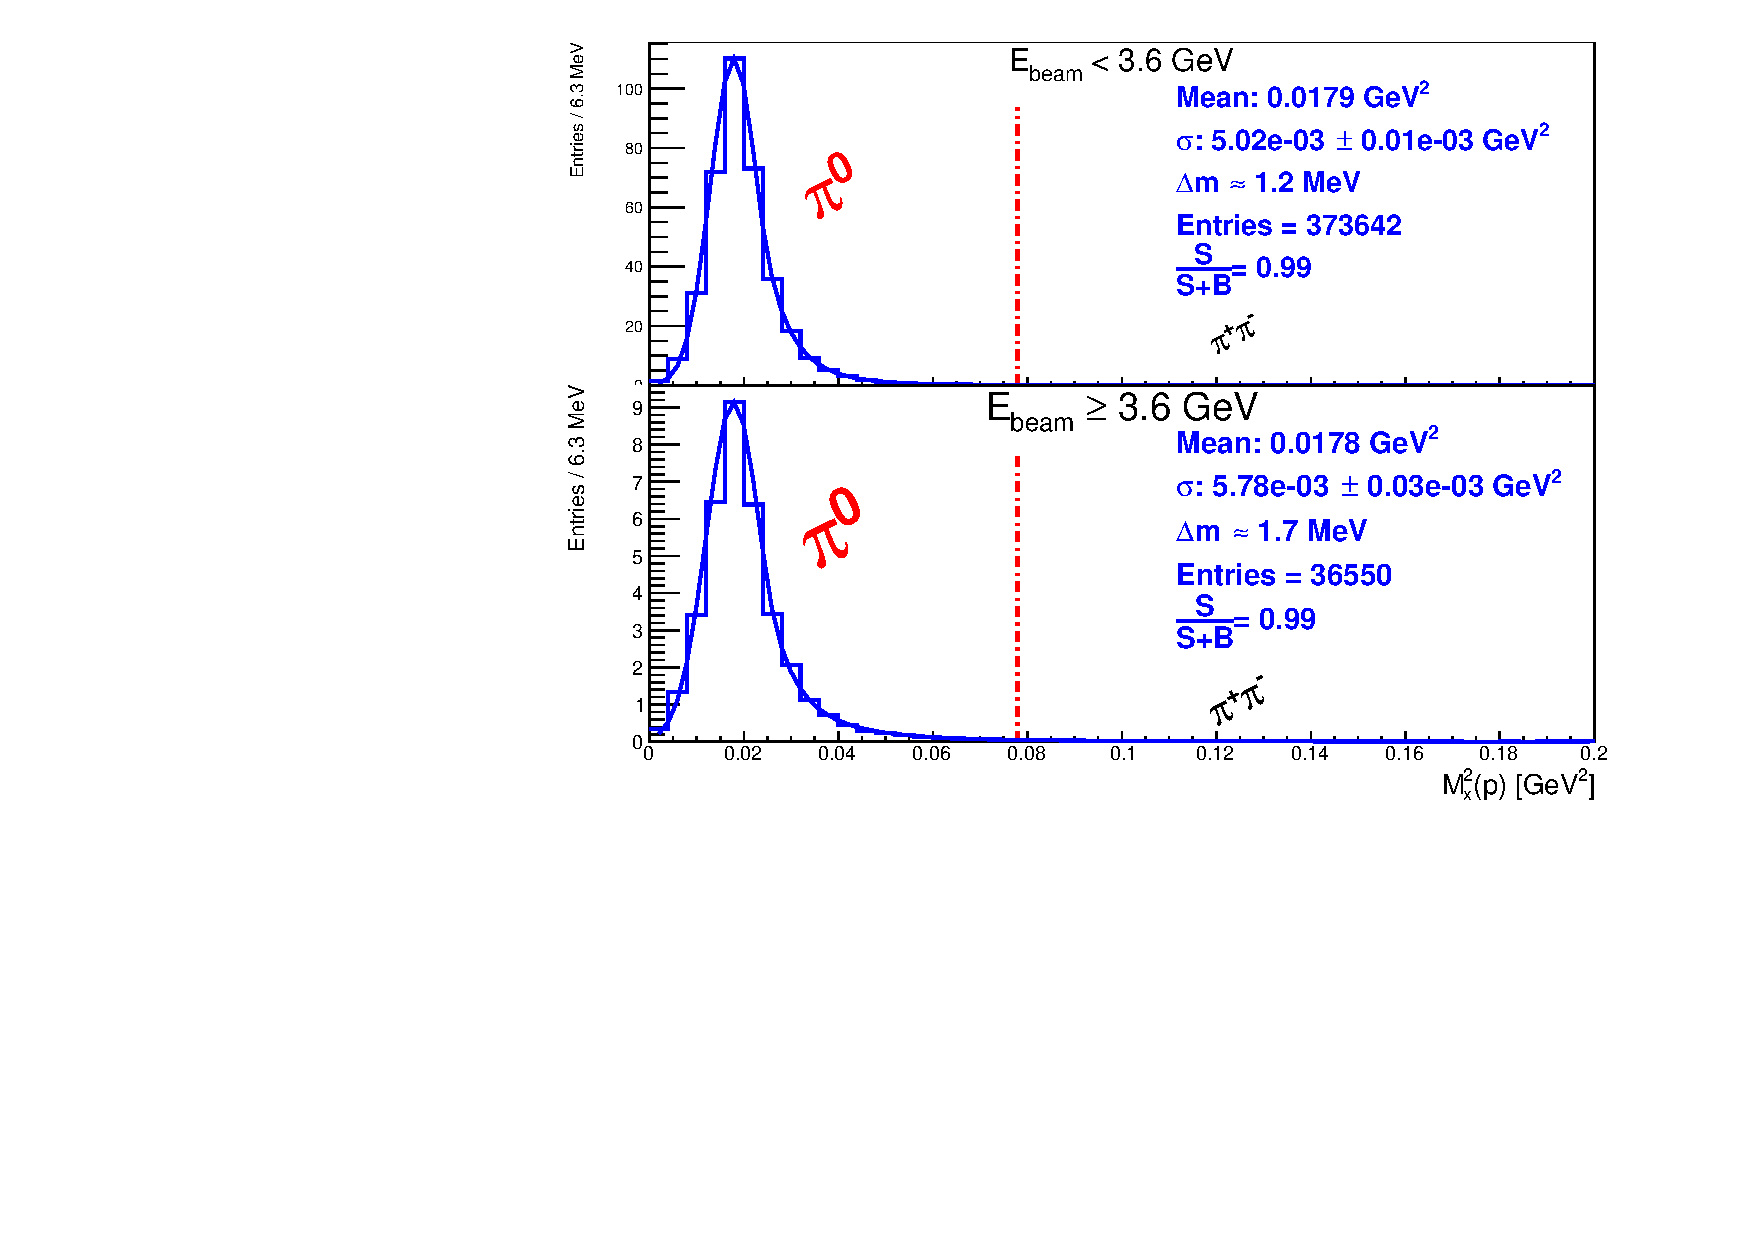
\includegraphics[width=\figwidth,height= 0.75 \hfigheight]{\figures/analysis/KineFitter/DATA/hdataLEP_MOR_pi0_FINAL_PLOTS.pdf}
\caption[Number of data events plotted vs. missing mass $M_x(\gamma p \to p X)$ for $\gamma p \to p e^+ e^- (\gamma)$ events after all cuts and corrections.]{\label{fig:kinfit.final.plot}Number of data events plotted vs. missing mass $M_x(\gamma p \to p X)$ for $\gamma p \to p e^+ e^- (\gamma)$ events after all cuts and corrections.}
\end{center}\end{figure}
\FloatBarrier

	\section{Target Density}\label{sec:analysis.target_density}

We need to know the target density to calculate the differential cross-section. The procedure for determining the density of $\ell$H$_2$ target in \abbr{CLAS} has already been established in~\cite{clas.target.density}. In the g12 experiment, the target temperature and pressure was measured periodically during each run. Each run contained at least 3 measurements of the pressure and temperature. The formula for calculating the target density is;
\begin{align}
\rho = a_1T^2 + a_2P +a_3 \label{eq:target_density} \ ,
\end{align} 
where $T$ and $P$ represent the temperature and pressure respectively and $a_1$, $a_2$, $a_3$ are constants given in Tab.~\ref{tab:targetdensity} taken from~\cite{mccarty}. Figure~\ref{fig:target_density} shows the average target density, $\bar \rho$, for each run along with the $\sqrt{\sigma^2}$.
\begin{table}[h!]
\begin{minipage}{\textwidth}
\begin{center}
\begin{singlespacing}

\caption[Target Density Constants]{\label{tab:targetdensity}Constants used in target density measurements \vspace{0.75mm}}

\begin{tabular}{c|c}

%\hline \hline
%
%operation & \multicolumn{3}{c}{Generation} \\
%charge & I & II & III \\

\hline
Parameter & Value \\
\hline

$a_{1}$ & $-2.89 \cdot 10^{-5} \frac{g}{cm^3K^2}$  \\
$a_{2}$ & $1.0 \cdot 10^{-7} \frac{g}{cm^3mbar}$  \\
$a_{3}$ & $8.249 \cdot 10^{-2} \frac{g}{cm^3}$  \\
\hline \hline
\end{tabular}

\end{singlespacing}
\end{center}
\end{minipage}
\end{table}
\vspace{20pt}
The average density, for each run, was calculated as;
\begin{align}
\bar \rho_{run} = \frac{1}{N}\sum_i^N \rho_i \ ,
\end{align} 
while the variance $\sigma^2$ is calculated, for each run, as;
\begin{align}
\sigma^2 = \frac{1}{N - 1}\sum_i^N (\rho_i - \bar \rho)^2 \ .
\end{align}
Once the target density was calculated for each run, the average target density for all g12 runs was calculated using;
\begin{align}
\bar \rho_{tot} = \frac{1}{N_{run}}\sum_i^{N_{run}} \bar \rho_{run} = 0.0711398 \pm 1.74 \cdot10^{-5}\ ,
\end{align} 
while the variance $\sigma^2$ is calculated, for all g12 run, as;
\begin{align}
\sigma_{tot}^2 = \frac{1}{N_{run} -1}\sum_i^{N_{run}} (\bar \rho_{run} - \bar \rho_{tot})^2 = 0.00024 \ .
\end{align}
Since the uncertainty, $\sigma$, in the target density is lower than the uncertainty of the physical in the target materials, the target density uncertainty will not be a factor in the total systematic errors, Sec.\ref{sec:results.systematics}. The target length has an inaccuracy of 40~cm $\pm$ 0.2~cm. This gives a systematic of 0.5\%. 

\begin{figure}[h!]\begin{center}
\includegraphics[width=\figwidth,height=\qfigheight]{\figures/analysis/TARGET_DENSITY/G12_Target_Density.pdf}
\caption[Target density for g12]{\label{fig:target_density}Target density for g12}
\end{center}\end{figure}
\FloatBarrier
	\section{Photon Normalization}\label{sec:analysis.gflux}
In the calculation of the differential cross-section, Sec.~\ref{sec:results}, accuracy of the total number of photons incident on the target will determine the accuracy of the cross-section measurement. The procedure for determining the total number of photons in CLAS has already been established in~\cite{clas.gflux} and is explained in Sec. 4 of ~\cite{g12note}. 
%
%
%This procedure was performed for the g12 data set and is discussed further in~\cite{clas.g12.note}. In this analysis, only events which were in the ``good'' scalar interval were considered. A ``good'' scalar interval relates to data recorded when the photon flux was recorded in ``live-time''. ``Live-time'' is the time that the data acquisition was ready to record events in conjunction with CLAS. For this analysis the photon flux, gflux, was binned in increments of 25~MeV and can be seen in Fig.~\ref{fig:gflux}.
A 25 MeV binning was chosen to compare past experiments differential cross-sections with this analysis.

It should be noted that beam energies with values $3.025 \pm 25$~MeV, $3.075 \pm25$~MeV, $3.125 \pm25$~MeV and $3.525 \pm25$~MeV bins are excluded from the analysis due to flux calculation problems that arose from dead scintillators in the tagger. 

\begin{figure}[h!]\begin{center}
\includegraphics[width=\figwidth,height= 0.75 \hfigheight]{\figures/analysis/GFLUX/Analysis_GFlux_II.pdf}
\caption[Photon flux for analysis]{\label{fig:gflux}Photon flux for analysis.}
\end{center}\end{figure}
\FloatBarrier

%\subsection{Gflux}
	\section{Fiducial Cut}\label{sec:results.fidcuts}
Fiducial cuts for g12 were derived and appropriately described in~\cite{g12note}. For this analysis, fiducial cuts were performed prior the the application of the track efficiency described in Sec.~\ref{sec:results.normalization}.
\section{Normalization}\label{sec:results.normalization}
\subsection{Normalization History}
In the g11 experiment there is an 18\% discrepancy between the differential cross-sections of $\gamma p \rightarrow p \omega$ measured channels $\gamma p \rightarrow p \pi^+ \pi^- (\pi^0)$ and $\gamma p \rightarrow p \pi^+ (\pi^- \pi^0)$. One method of correction for this effect was to apply a global scale factor to the two track topology. The scale factor was on the order of 18\%. The cause of the inefficiency was unknown but is believed to be due to the high current of the electron beam in conjunction with requiring 3 charged tracks from a 2-prong trigger.
\subsection{g12 Normalization Procedure}\label{sec:results.g12normalization}
In this analysis, a normalization constant on the order of 18\% was also needed. The cause of this effect is unknown, but it is also believed to be related to using 3 charged tracks from 2-prong triggers at high current. \abbr{GPP} is responsible for smearing and dropping inefficient parts of the detector but not trigger efficiency. Therefore the normalization could be simulated if it was a trigger effect or another happenstance related to requiring 3 charged tracks in the analysis. To investigate this effect the following 3 topologies; 
\begin{align}\label{eq:eff_topologies}
\gamma p \rightarrow p \pi^+ (\pi^-) \nonumber\\
\gamma p \rightarrow p \pi^- (\pi^+)  \nonumber\\
\gamma p \rightarrow \pi^+ \pi^- (p)
\end{align}  
were skimmed from data and simulated using the prescription chain in Sec.~\ref{sec:analysis.simulation}. In order to eliminate any statistical effects, $\frac{1}{4}$ of the entire g12 data set was used and over 1 billion events were generated for simulation. Table~\ref{tab:eff_events} lists the number of events analyzed for each of the topologies listed in Eq.~\ref{eq:eff_topologies}.
\begin{table}[h!]
\begin{minipage}{\textwidth}
\begin{center}
\begin{singlespacing}

\caption[Number of Events Used in Efficiency Study]{\label{tab:eff_events}Number of Events Used in Efficiency Study \vspace{0.75mm}}

\begin{tabular}{c|c|c}

\hline
Topology & Data Reconstructed & Monte-Carlo Generated/Reconstructed \\
\hline
$\gamma p \rightarrow p \pi^+ (\pi^-)$ & $5.09\cdot10^{10}$ & $1.2\cdot10^9$ / $2.16\cdot10^8$ \\
$\gamma p \rightarrow p \pi^- (\pi^+)$ & $5.43\cdot10^{10}$ & $1.2\cdot10^9$ / $2.17\cdot10^8$ \\
$\gamma p \rightarrow \pi^+ \pi^- (p)$ & $5.34\cdot10^{10}$ & $1.2\cdot10^9$ / $1.08\cdot10^8$ \\
\hline \hline
\end{tabular}

\end{singlespacing}
\end{center}
\end{minipage}
\end{table}
\vspace{20pt}
The data had two orders of magnitude higher statistics than the simulation, this was done to ensure enough events to analyze in the high momentum spectrum. The simulation generated the listed reactions in phase space using PLUTO++~\cite{PLUTO}. The data and simulation were analyzed in the same manner.

The data was skimmed under the conditions of Eq.~\ref{eq:eff_topologies}. If the missing particle (particle in parenthesis) was detected, then this information was also recorded. After the data was skimmed, kinematic fits (1-C) were performed to the missing particles. Nominal geometric fiducial cuts were employed for all detected particles along with a pull probability for each topology  $>1~\%$, see Fig.~\ref{fig:eff_pull}.
\begin{figure}[h!]\begin{center}
\includegraphics[width=1.1 \figwidth,height=\hfigheight]{\figures/analysis/EFFICIENCY/All_Pull_Eff_Plot.pdf}
\caption[Number of events vs. the pull distribution for the reactions used in the normalization study for data]{\label{fig:eff_pull}Number of events vs. the 1-C pull probability distribution for the reactions used in the normalization study for data.}
\end{center}\end{figure}
\begin{figure}[h!]\begin{center}
\includegraphics[width=1.1 \figwidth,height=\hfigheight]{\figures/analysis/EFFICIENCY/All_Pull_Eff_PlotMC.pdf}
\caption[Number of events vs. the pull distribution for the reactions used in the normalization study for \abbr{MC}]{\label{fig:eff_pullMC} Number of events vs. the 1-C pull probability distribution for the reactions used in the normalization study for \abbr{MC}.}
\end{center}\end{figure}


The z-vertex of the two needed particles was determined by the method of distance of closest approach of the two vectors. The data was then binned for the fitted missing particle according to the z-vertex position, momentum, $\theta \sin\phi$, and $\theta \cos\phi$. The z-vertex and momentum binning used can be seen in Table~\ref{tab:eff_binning}. If the particle to be fit was detected by \abbr{CLAS}, the information was also binned according $z$-vertex, momentum, $\theta \sin\phi$, and $\theta \cos\phi$. However to ensure that the detected particle and the fitted missing particle were the same, the detected particle must have been in the same momentum bin as the fitted missing particle.
%\begin{table}[h!]
%{
%\centering
%\begin{minipage}{\textwidth}
%%\begin{center}
%\begin{singlespacing}
%
%\caption[Binning Used in Efficiency Study]{\label{tab:eff_binning}Binning Used in Efficiency Study \vspace{0.75mm}}
%
%
%\begin{tabular}{c||c|||c||c} \hline
%%%%%%% Title row starts here
%z bins~cm& Momentum bins~GeV & z bins~cm & Momentum bins~GeV \\ \hline
%%%%%%% Row Foo starts here
%$-105 \textless \ z \ \textless -110$ &
%\begin{tabular}{c}
% 0 - 0.5 \\ 0.5 - 0.75 \\ 0.75 - 1 \\ 1 - 1.5 \\ 1.5 - 2  \\2 - 2.5 \\2.5 - 3 \\3 - 5 
%\end{tabular} &
%$-100 \textless \ z \ \textless -105$ &
%\begin{tabular}{c}
% 0 - 0.5 \\ 0.5 - 0.75 \\ 0.75 - 1 \\ 1 - 1.5 \\ 1.5 - 2  \\2 - 2.5 \\2.5 - 3 \\3 - 5 
%\end{tabular} \\ \hline \hline \hline
%%
%%
%z bins~cm& Momentum bins~GeV & z bins~cm & Momentum bins~GeV \\ \hline
%%%%%%% Row Foo starts here
%$-100 \textless \ z \ \textless -95$ &
%\begin{tabular}{c}
% 0 - 0.5 \\ 0.5 - 0.75 \\ 0.75 - 1 \\ 1 - 1.5 \\ 1.5 - 2  \\2 - 2.5 \\2.5 - 3 \\3 - 5 
%\end{tabular} &
%$-95 \textless \ z \ \textless -90$ &
%\begin{tabular}{c}
% 0 - 0.5 \\ 0.5 - 0.75 \\ 0.75 - 1 \\ 1 - 1.5 \\ 1.5 - 2  \\2 - 2.5 \\2.5 - 3 \\3 - 5 
%\end{tabular} \\ \hline \hline \hline
%%
%%
%%
%z bins~cm& Momentum bins~GeV & z bins~cm & Momentum bins~GeV \\ \hline
%%%%%%% Row Foo starts here
%$-90 \textless \ z \ \textless -85$ &
%\begin{tabular}{c}
% 0 - 0.5 \\ 0.5 - 0.75 \\ 0.75 - 1 \\ 1 - 1.5 \\ 1.5 - 2  \\2 - 2.5 \\2.5 - 3 \\3 - 5 
%\end{tabular} &
%$-85 \textless \ z \ \textless -80$ &
%\begin{tabular}{c}
% 0 - 0.5 \\ 0.5 - 0.75 \\ 0.75 - 1 \\ 1 - 1.5 \\ 1.5 - 2  \\2 - 2.5 \\2.5 - 3 \\3 - 5 
%\end{tabular} \\ \hline \hline \hline
%%
%%
%%
%z bins~cm& Momentum bins~GeV & z bins~cm & Momentum bins~GeV \\ \hline
%%%%%%% Row Foo starts here
%$-80 \textless \ z \ \textless -75$ &
%\begin{tabular}{c}
% 0 - 0.5 \\ 0.5 - 0.75 \\ 0.75 - 1 \\ 1 - 1.5 \\ 1.5 - 2  \\2 - 2.5 \\2.5 - 3 \\3 - 5 
%\end{tabular} &
%$-75 \textless \ z \ \textless -70$ &
%\begin{tabular}{c}
% 0 - 0.5 \\ 0.5 - 0.75 \\ 0.75 - 1 \\ 1 - 1.5 \\ 1.5 - 2  \\2 - 2.5 \\2.5 - 3 \\3 - 5 
%\end{tabular} \\ \hline \hline
%
%%Foo &
%%\begin{tabular}{c} 1 \\ 2 \\ 3 \\ 4 \\
%%\end{tabular} &
%%\begin{tabular}{c} 2 \\ 5 \\ 9 \\ 8 \\
%%\end{tabular} \\ \hline \hline
%%
%%%%%%%% Row Bar starts here
%%Bar &
%%\begin{tabular}{c} 1 \\ 2 \\ 3 \\ 4 \\
%%\end{tabular} &
%%\begin{tabular}{c} 31 \\ 23 \\ 16 \\ 42 \\
%%\end{tabular} \\ \hline
%\end{tabular}
%
%
%\end{singlespacing}
%%\end{center}
%\end{minipage}
%}
%\end{table}
%

\begin{table}[h!]
\begin{minipage}{\textwidth}
\begin{center}
\begin{singlespacing}

\caption[Binning Used in Efficiency Study]{\label{tab:eff_binning}Binning Used in Efficiency Study \vspace{0.75mm}}


\begin{tabular}{c||c} \hline
%%%%%% Title row starts here
z bins~[cm] (5~cm \ increments)& Momentum bins~[GeV]  \\ \hline
%%%%%% Row Foo starts here
$-70~\mathrm{cm} \textless \ z \ \textless -110~\mathrm{cm} $  &
\begin{tabular}{c}
 0 - 0.5 \\ 0.5 - 0.75 \\ 0.75 - 1 \\ 1 - 1.5 \\ 1.5 - 2  \\2 - 2.5 \\2.5 - 3 \\3 - 5 
\end{tabular} \\ \hline \hline 

\end{tabular}

\end{singlespacing}
\end{center}
\end{minipage}
\end{table}
\vspace{20pt}
The $\theta \sin\phi$ and $\theta \cos\phi$ binning was chosen to interpret the geometric x and y space the particle travels, independent of momentum and x and y vertex. These $\theta \sin\phi$ and $\theta \cos\phi$ quantities are plotted as x and y variable of a histogram. To better illustrate this interpretation consider a spherical coordinate system where;
\begin{align}
r=\sqrt{x^2 + y^2 + z^2} \\
x = r\sin\theta\cos\phi \\
y = r\sin\theta\sin\phi
\end{align}
therefore,
\begin{align}
\theta \sin\phi = \left(\frac{\theta}{r\sin\theta}\right)y \label{eq:sin1} \\
\theta \cos\phi = \left(\frac{\theta}{r\sin\theta}\right)x \label{eq:sin2} \ .
\end{align}
It can be seen that plotting Eq~\ref{eq:sin2} versus Eq~\ref{eq:sin1} projects $x-y$ space.

For each type of missing particle, we plotted the number of events versus $\theta \sin\phi$ and $\theta \cos\phi$. We then plotted the number of events where the ``missing" particle was detected. The ratio of the number of detected ``missing" particle to the total number of ``missing" particles is the detection efficiency for that bin in $z$-vertex, p, $\theta \sin\phi$ and $\theta \cos\phi$ (see Figs~\ref{fig:eff_prot_data},~\ref{fig:eff_pip_data} and~\ref{fig:eff_pim_data}). This process was repeated for simulated data (see Figs~\ref{fig:eff_prot_MC},~\ref{fig:eff_pip_MC} and~\ref{fig:eff_pim_MC}). The ratio of the simulated efficiency to the measured efficiency for each particle was used to correct the data (see Figs~\ref{fig:toteff_prot},~\ref{fig:toteff_pip} and~\ref{fig:toteff_pim}). This procedure revealed any differences between the real and simulated detector responses.
\FloatBarrier
\subsection{g12 Normalization Results}

It was noticed that the simulation was over-efficient as compared to the data and the ratio of the efficiency of reconstruction should suffice as a correction to the data. Figures~\ref{fig:eff_prot_data},~\ref{fig:eff_pip_data},~\ref{fig:eff_pim_data} depict the efficiency of data reconstruction for the proton $\pi^+$ and $\pi^-$ respectively. Figures~\ref{fig:eff_prot_MC},~\ref{fig:eff_pip_MC},~\ref{fig:eff_pim_MC} depict the efficiency of the simulation reconstruction for the proton $\pi^+$ and $\pi^-$ respectively. Figures~\ref{fig:toteff_prot},~\ref{fig:toteff_pip},~\ref{fig:toteff_pim} depict the over-efficiency of the simulation to data reconstruction for the proton $\pi^+$ and $\pi^-$ respectively.
The total over-efficiency was calculated as the product of each track's over-efficiency, i.e.,
\begin{align}\label{eq:eff_tot}
\epsilon = \epsilon_{proton}\cdot\epsilon_{\pi^+}\cdot\epsilon_{\pi^-}.
\end{align}
The value of $\epsilon$ from Eq.~\ref{eq:eff_tot} is the same quantity used in the cross-section calculation in Eq.~\ref{eq:xsection1}.
	% % %PROT
\begin{figure}[h!]\begin{center}
		\includegraphics[width=1.1 \figwidth,height=\hfigheight]{\figures/analysis/EFFICIENCY/Prot_Thesis_EffData_Plot.pdf}
		\caption[$\theta \cos\phi$ vs. $\theta \sin\phi$ plot showing the efficiency of detecting the proton with z-vertex $-90\textless z\textless-85$~cm and momentum $0.75\textless p \textless 1$~GeV from a 2 charged track reaction using \abbr{CLAS} detection for g12]{\label{fig:eff_prot_data} $\theta \cos\phi$ vs. $\theta \sin\phi$ plot showing the efficiency of detecting the proton with z-vertex $-90\textless z\textless-85$~cm and momentum $0.75\textless p \textless 1$~GeV from a 2 charged track reaction using \abbr{CLAS} detection for g12.}
\end{center}\end{figure}
	%
\begin{figure}[h!]\begin{center}
		\includegraphics[width=1.1 \figwidth,height=\hfigheight]{\figures/analysis/EFFICIENCY/Prot_Thesis_EffMC_Plot.pdf}
		\caption[$\theta \cos\phi$ vs. $\theta \sin\phi$ plot showing the efficiency of reconstructing the proton with z-vertex $-90\textless z\textless-85$~cm and momentum $0.75\textless p \textless 1$~GeV from a 2 charged track reaction using \abbr{CLAS} Monte-Carlo for g12]{\label{fig:eff_prot_MC} $\theta \cos\phi$ vs. $\theta \sin\phi$ plot showing the efficiency of reconstructing the proton with z-vertex $-90\textless z\textless-85$~cm and momentum $0.75\textless p \textless 1$~GeV from a 2 charged track reaction using \abbr{CLAS} Monte-Carlo for g12.}
\end{center}\end{figure}
		%
\begin{figure}[h!]\begin{center}
		\includegraphics[width=1.1 \figwidth,height=\hfigheight]{\figures/analysis/EFFICIENCY/Prot_Thesis_TotEff_Plot.pdf}
		\caption[$\theta \cos\phi$ vs. $\theta \sin\phi$ plot showing the over-efficiency of simulating the proton with z-vertex $-90\textless z\textless-85$~cm and momentum $0.75\textless p \textless 1$~GeV from a 2 charged track reaction]{\label{fig:toteff_prot} $\theta \cos\phi$ vs. $\theta \sin\phi$ plot showing the over-efficiency of simulating the proton with z-vertex $-90\textless z\textless-85$~cm and momentum $0.75\textless p \textless 1$~GeV from a 2 charged track reaction.}
\end{center}\end{figure}
			% % %PIP
\begin{figure}[h!]\begin{center}
		\includegraphics[width=1.1 \figwidth,height=\hfigheight]{\figures/analysis/EFFICIENCY/Pip_Thesis_EffData_Plot.pdf}
		\caption[$\theta \cos\phi$ vs. $\theta \sin\phi$ plot showing the efficiency of detecting the $\pi^+$ with z-vertex $-90\textless z\textless-85$~cm and momentum $0.75\textless p \textless 1$~GeV from a 2 charged track reaction using \abbr{CLAS} detection for g12]{\label{fig:eff_pip_data} $\theta \cos\phi$ vs. $\theta \sin\phi$ plot showing the efficiency of detecting the $\pi^+$ with z-vertex $-90\textless z\textless-85$~cm and momentum $0.75\textless p \textless 1$~GeV from a 2 charged track reaction using \abbr{CLAS} detection for g12.}
\end{center}\end{figure}
				%
\begin{figure}[h!]\begin{center}
		\includegraphics[width=1.1 \figwidth,height=\hfigheight]{\figures/analysis/EFFICIENCY/Pip_Thesis_EffMC_Plot.pdf}
		\caption[$\theta \cos\phi$ vs. $\theta \sin\phi$ plot showing the efficiency of reconstructing the $\pi^+$ with z-vertex $-90\textless z\textless-85$~cm and momentum $0.75\textless p \textless 1$~GeV from a 2 charged track reaction using \abbr{CLAS} Monte-Carlo for g12]{\label{fig:eff_pip_MC} $\theta \cos\phi$ vs. $\theta \sin\phi$ plot showing the efficiency of reconstructing the $\pi^+$ with z-vertex $-90\textless z\textless-85$~cm and momentum $0.75\textless p \textless 1$~GeV from a 2 charged track reaction using \abbr{CLAS} Monte-Carlo for g12.}
\end{center}\end{figure}
					%
\begin{figure}[h!]\begin{center}
		\includegraphics[width=1.1 \figwidth,height=\hfigheight]{\figures/analysis/EFFICIENCY/Pip_Thesis_TotEff_Plot.pdf}
		\caption[$\theta \cos\phi$ vs. $\theta \sin\phi$ plot showing the over-efficiency of simulating the $\pi^+$ with z-vertex $-90\textless z\textless-85$~cm and momentum $0.75\textless p \textless 1$~GeV from a 2 charged track reaction]{\label{fig:toteff_pip} $\theta \cos\phi$ vs. $\theta \sin\phi$ plot showing the over-efficiency of simulating the $\pi^+$ with z-vertex $-90\textless z\textless-85$~cm and momentum $0.75\textless p \textless 1$~GeV from a 2 charged track reaction.}
\end{center}\end{figure}
						% % %PIM
\begin{figure}[h!]\begin{center}
		\includegraphics[width=1.1 \figwidth,height=\hfigheight]{\figures/analysis/EFFICIENCY/Pim_Thesis_EffData_Plot.pdf}
		\caption[$\theta \cos\phi$ vs. $\theta \sin\phi$ plot showing the efficiency of detecting the $\pi^-$ with z-vertex $-90\textless z\textless-85$~cm and momentum $0.75\textless p \textless 1$~GeV from a 2 charged track reaction using \abbr{CLAS} detection for g12]{\label{fig:eff_pim_data} $\theta \cos\phi$ vs. $\theta \sin\phi$ plot showing the efficiency of detecting the $\pi^-$ with z-vertex $-90\textless z\textless-85$~cm and momentum $0.75\textless p \textless 1$~GeV from a 2 charged track reaction using \abbr{CLAS} detection for g12.}
\end{center}\end{figure}
							%
\begin{figure}[h!]\begin{center}
		\includegraphics[width=1.1 \figwidth,height=\hfigheight]{\figures/analysis/EFFICIENCY/Pim_Thesis_EffMC_Plot.pdf}
		\caption[$\theta \cos\phi$ vs. $\theta \sin\phi$ plot showing the efficiency of reconstructing the $\pi^-$ with z-vertex $-90\textless z\textless-85$~cm and momentum $0.75\textless p \textless 1$~GeV from a 2 charged track reaction using \abbr{CLAS} Monte-Carlo for g12]{\label{fig:eff_pim_MC} $\theta \cos\phi$ vs. $\theta \sin\phi$ plot showing the efficiency of reconstructing the $\pi^-$ with z-vertex $-90\textless z\textless-85$~cm and momentum $0.75\textless p \textless 1$~GeV from a 2 charged track reaction using \abbr{CLAS} Monte-Carlo for g12.}
\end{center}\end{figure}
								%
\begin{figure}[h!]\begin{center}
		\includegraphics[width=1.1 \figwidth,height=\hfigheight]{\figures/analysis/EFFICIENCY/Pim_Thesis_TotEff_Plot.pdf}
		\caption[$\theta \cos\phi$ vs. $\theta \sin\phi$ plot showing the over-efficiency of simulating the $\pi^-$ with z-vertex $-90\textless z\textless-85$~cm and momentum $0.75\textless p \textless 1$~GeV from a 2 charged track reaction]{\label{fig:toteff_pim} $\theta \cos\phi$ vs. $\theta \sin\phi$ plot showing the over-efficiency of simulating the $\pi^-$ with z-vertex $-90\textless z\textless-85$~cm and momentum $0.75\textless p \textless 1$~GeV from a 2 charged track reaction.}
\end{center}\end{figure}
\FloatBarrier
%
\subsection{Normalization Comparison}
To validate the g12 normalization results, the g12 $\pi^0$ differential cross-section was calculated using the G11 global normalization factor and then compared to the g12 $\pi^0$ differential cross-section using the g12 normalization procedure results. It is shown in Fig.~\ref{fig:toteff_compareI} and Fig.~\ref{fig:toteff_compareII} that the 2 methods agree with one another except for the very forward regions of $\cos\theta^{\pi^0}_{C.M.}$, where the cross-section using the dynamic normalization is larger than the cross-section measured with the G11 global normalization, however the larger cross-sections at forward $\cos\theta^{\pi^0}_{C.M.}$ agree very well with the past results of~\cite{ELSA11}.

\begin{figure}[h!]\begin{center}
\includegraphics[width=1.1 \figwidth,height=\hfigheight]{\figures/analysis/EFFICIENCY/G12_XSection_Normaization_Compare_thesisI.pdf}
\caption[$\frac{d \sigma}{d \Omega}$ vs. $\cos \theta$ plot showing the g12 \pizT differential cross-section when the G11 global normalization is used (blue) and when the g12 dynamic normalization is used (red) for various bins of beam energy inside lepton trigger acceptance]{\label{fig:toteff_compareI} $\frac{d \sigma}{d \Omega}$ vs. $\cos \theta$ plot showing the g12 \pizT differential cross-section when the G11 global normalization is used (blue) and when the g12 dynamic normalization is used (red) for various bins of beam energy inside the lepton trigger acceptance.}
\end{center}\end{figure}

\begin{figure}[h!]\begin{center}
\includegraphics[width=1.1 \figwidth,height=\hfigheight]{\figures/analysis/EFFICIENCY/G12_XSection_Normaization_Compare_thesisII.pdf}
\caption[$\frac{d \sigma}{d \Omega}$ vs. $\cos \theta$ plot showing the g12 \pizT differential cross-section when the G11 global normalization is used (blue) and when the g12 dynamic normalization is used (red) for various bins of beam energy above \abbr{MORB} threshold]{\label{fig:toteff_compareII} $\frac{d \sigma}{d \Omega}$ vs. $\cos \theta$ plot showing the g12 \pizT differential cross-section when the G11 global normalization is used (blue) and when the g12 dynamic normalization is used (red) for various bins of beam energy above the \abbr{MORB} threshold.}
\end{center}\end{figure}

\FloatBarrier

\subsection{Normalization Uncertainties}
The statistical uncertainties of the normalization correction was minimized by ensuring that the statistical sample of the data and \abbr{MC} was sufficient in each bin of $z$-vertex, momentum, $\theta \sin\phi$ and $\theta \cos\phi$. The maximum statistical uncertainty was 0.01\%. The systematic uncertainties of the normalization correction was calculated and shown in Sec.~\ref{sec:trkeffuncert}.
    \section{Simulation}\label{sec:analysis.simulation}
There are certain kinematic regions of \abbr{CLAS} in which physics events are not being recorded properly i.e.~the area dividing each sector in \abbr{CLAS}. Furthermore each sector in \abbr{CLAS} is asymmetric in the acceptance of events due to subsystem inefficiencies such as inoperable \abbr{DC} wires, \abbr{PMT} inefficiencies, dead scintillator strips the the \abbr{TOF} and \abbr{ST} subsystems. When a triggered event is recorded and reconstructed these asymmetric inefficiencies factors are reflected and must be carefully understood because these factors are properties of the \abbr{CLAS} detector and independent of any physics that occurred. To properly understand the detector effects on the data, \abbr{CLAS} utilizes a \abbr{GEANT} simulation package know as \abbr{GSIM}. To prepare an event for \abbr{GSIM} the program \abbr{GAMP2PART} converts a text file, containing the 4-momentum of the generated event, into a suitable file format for \abbr{GSIM}. \abbr{GSIM} then simulates the passage of these particles through the \abbr{CLAS} detector and generates the associated \abbr{ADC} and \abbr{TDC} information from detector hits. \abbr{GSIM} takes into account detector inefficiencies described in the \abbr{\texttt{CLAS\_CALDB\_RUNINDEX}}. The \abbr{CLAS\_CALDB\_RUNINDEX} is an array of information about each subsystem's inefficiency that was derived during the g12 calibration process. The \abbr{GSIM} simulated hits are then ``post-processed'' by smearing the \abbr{TDC} and \abbr{ADC} hits to imitate the observed resolution of the detector subsystems using the program \abbr{GPP} (\abbr{GSIM} post-processor). \abbr{GPP} also removes detector hits due to inefficient \abbr{DC} wires. The simulation output processed with \abbr{GPP} is then reconstructed with \texttt{a1c}, the same program used to reconstruct data events. The reconstructed simulation is subject to the same scrutiny as real data events, undergoing all the cuts (Sec.~\ref{sec:analysis.data.reduction}), corrections (Sec.~\ref{sec:analysis.corrections}), and kinematic fitting (Sec.~\ref{sec:analysis.fitting}), as the real data except for beam corrections (Sec.~\ref{sec:analysis.corrections.beam}).
\subsection{Simulation Verification}\label{sec:analysis.accept.verify}
Part of understanding the simulation output is understanding how well the simulation mimics the real data. To investigate this, 26,000 real \epemT events were treated as generated events and inputted into the \\ \abbr{GAM2PART}$\to$\abbr{GSIM}$\to$\abbr{GPP}$\to$\texttt{a1c}
\\ chain. Of the 26,000 events, only 100 were successfully reconstructed through the simulation chain. The source of this low efficiency was due to the calibrations entries for the \abbr{CC} and \abbr{EC} in the \abbr{CLAS\_CALDB\_RUNINDEX} not having values in which would set the ``PEDESTAL'' values appropriately for simulation. The calibrations constants in the \abbr{CLAS\_CALDB\_RUNINDEX} were correct for data reconstruction, but not for simulation reconstruction of \epemT in the \abbr{CC} and \abbr{EC} subsystems. It was also discovered that the \abbr{CC} and \abbr{EC} subsystems should be simulated with ``RUN 10'' constants instead of the normal ``RUN 56855'' used by the g12 group. ``RUN 56855'' is a special run benchmarked to have the best calibrations and required to properly simulate the \abbr{ST}, \abbr{DC}, and \abbr{TOF} subsystems. To rectify this, a special \abbr{CLAS\_CALDB\_RUNINDEX} was created, changing ``RUN 10'' to have ``RUN 56855'' constants for all subsystems except the \abbr{CC} and \abbr{EC} subsystems which were kept at ``RUN 10'' constants. Inputting the 26,000 real \epemT events into the simulation chain using the \abbr{CLAS\_CALDB\_RUNINDEX} \emph{RunIndexg12\_mk} outputted $\approx$~24,700 \epemT reconstructed events, i.e. $\approx$~95~\% efficiency.

The missing 5~\% was a result of ``time-based'' and ``hit-based'' tracking failures. The events that failed ``hit-based'' tracking contributes a 3.75~\% overall event inefficiency. The cause of the ``hit-based'' failure was never determined, but it was thought to have also occurred in the cooking of the data. Therefore since it did occur in the data reconstruction, this was considered to cancel the inefficiency of the simulation.

The ``time-based'' failure was due to a random bug in the processing of the \abbr{TDC} element information of \abbr{ST} (\abbr{STN0}) and the \abbr{ADC} element information of \abbr{ST} (\abbr{STN1}) raw data banks. The bug miscalculated the tracks sector exiting the \abbr{ST} even as the hit element of the \abbr{ST} matched that to the track in the \abbr{DC}. If the track failed due to this error, it usually passed ``time-based'' on the second or third pass of the ``time-based'' tracking if another particle passed ``time-based'' during the initial pass. The probability that a track failed initial ``time-based" tracking was $\approx$~.23\%. The probability that this failed event would pass ``time-based" tracking after another pass was $\approx99.78\%$. The average inefficiency for three charged track events for data was 0.0125\%

%This inefficiency depends on the distance the track is from the z-vertex position and can be seen in Fig.~\ref{fig:classt.ineffII}.
%\begin{figure}[h!]\begin{center}
%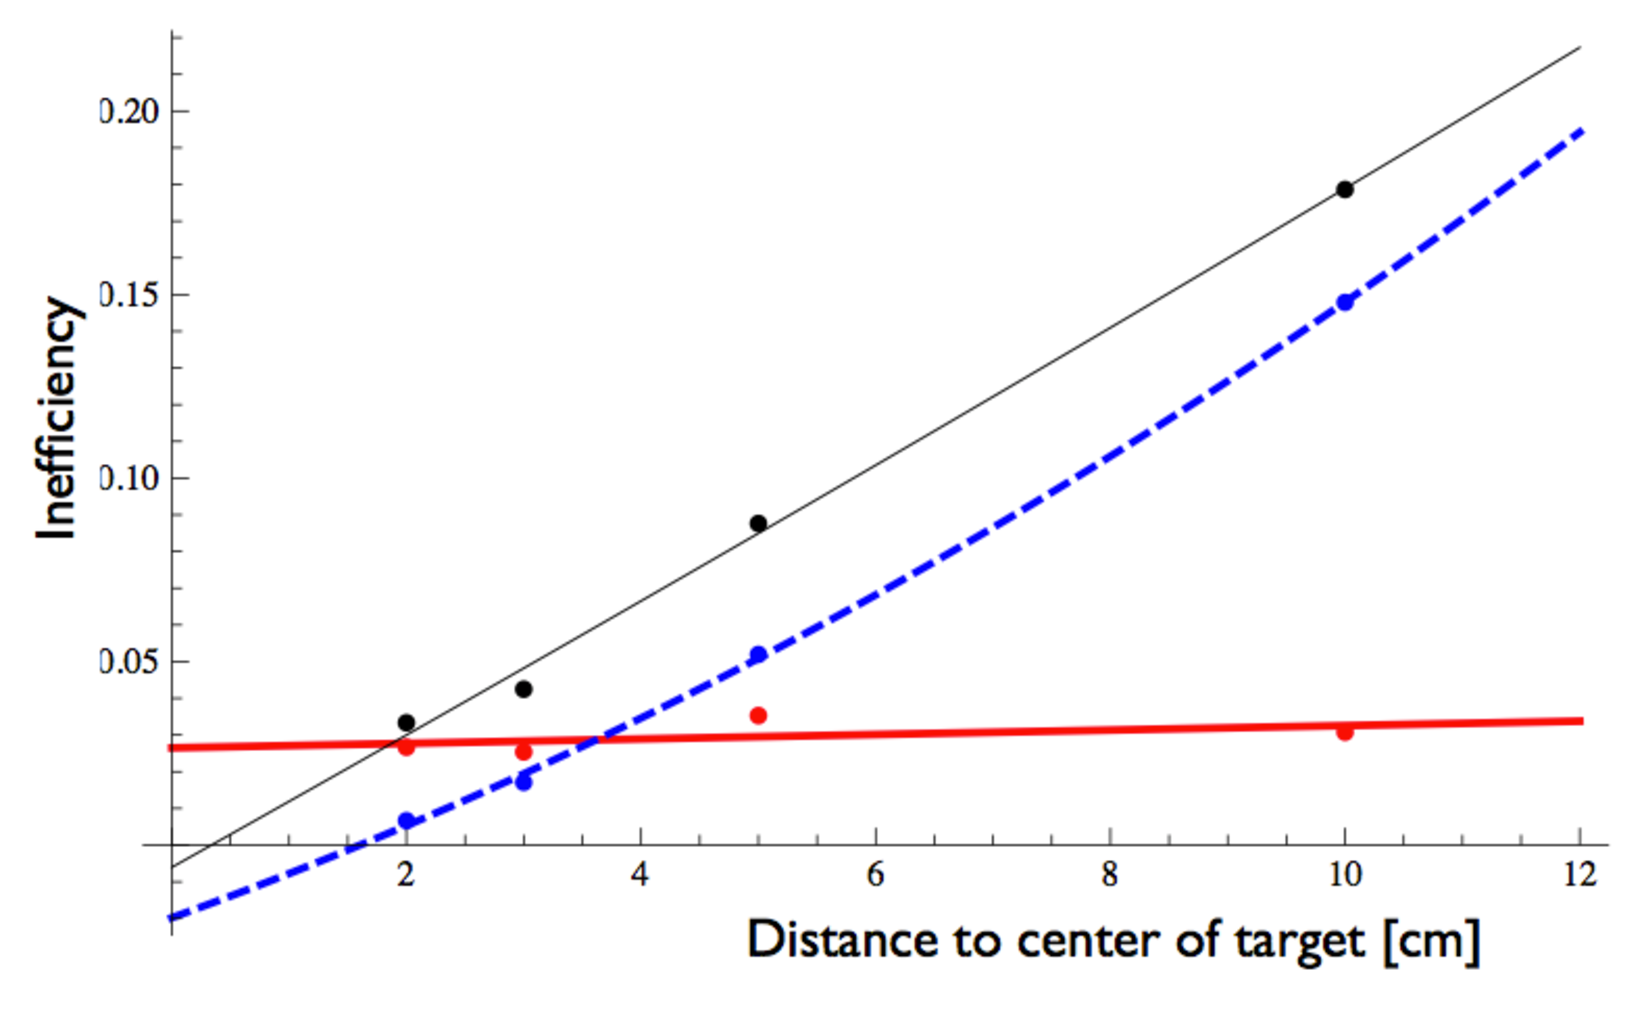
\includegraphics[width=0.8\figwidth,height=0.7\qfigheight]{\grpath/hall-b/st_issue_4_thesis.pdf}
%\caption[Start Counter Inefficiency]{\label{fig:classt.ineffII}{\coloronline}Plot showing the inefficiency of the start counter from data events, red-solid line is the inefficiency of reconstruction based solely on hit-based tracking, blue-dashed line is inefficiency of start counter, black-solid is combined. }
%\end{center}\end{figure}

\FloatBarrier
\subsection{PLUTO++ Event Generator}\label{sec:pluto}

Pluto~\cite{PLUTO} is a Monte-Carlo event generator designed for the study of hadronic interactions and heavy ion reactions in \abbr{HADES}, \abbr{FAIR} and upcoming \abbr{PANDA} collaborations. The versatility of Pluto enables its use as an event generator for photoproduction in \abbr{CLAS}. For hadronic interactions, Pluto can generate interactions from pion production threshold to intermediate energies of a few~GeV per nucleon. The entire software package is based on ROOT and uses ROOT's embedded C++ interpreter to control the generation of events. Programming event reaction can be set up with a few lines of ROOT macro code without detailed knowledge of programming. Some features in Pluto are, but not limited to;
\begin{itemize}
	\item Ability to generate events in phase space.
	\item Ability to generate events with a continuous bremsstrahlung photon beam.
	\item Ability to generate events weighted by a user defined $t$-slope.
	\item Ability to generate events weighted by a user defined cross-section.
	\begin{itemize}
		\item Total cross section can be inputted via functional form or histogram.
		\item Differential cross sections can be inputted via functional forms or histograms for specific beam energies up to 110 histograms relating to intervals of beam energy.
	\end{itemize}
	\item Ability to generate events that decay via already established physics parameters, i.e.~transition form factors.
	\item Ability to generate events that decay via modified established physics parameters.
	\item Ability to generate events with multiple production channels, weighted by user inputted cross-section probability.
	\item Ability to generate events with multiple decay channels, weighted by user inputted branching ratio.
	\item Ability to perform vertex smearing.
	\item Ability to create virtual detectors.
\end{itemize}

For the analysis presented in this work, Pluto was used in conjunction with known differential cross sections to verify simulation momentum smearing and tagger resolution, Sec.~\ref{sec:analysis.simsmear.verify}. Pluto was also utilized as a phase space generator in this analysis, to perform a ``tune'' on the kinematic fitter, Sec.~\ref{sec:analysis.fitting}, to calculate the acceptance corrections Sec.~\ref{sec:results.acceptance}, and to calculate the normalization Sec.~\ref{sec:results.normalization}.

\subsection{Simulating the Lepton Trigger}\label{sec:analysis.accept.trigger}
During the collection process, for an event to be written by the \abbr{DAQ} it must have passed at least one of the trigger ``bits" defined in Sec.~\ref{sec:clas.g12.conditions.data}. As discussed in Sec.~\ref{sec.data.trig.lepton}, the process of lepton triggering required a coincidence between the \abbr{EC} and the \abbr{CC} subsystems. This coincidence was established by using the voltage sum of the \abbr{CC} for a sector and the voltage sum of the \abbr{EC} for the same sector and comparing each sum to a preset threshold described in Table~\ref{tab:data.ecccthresh}. However when \abbr{GSIM} simulates tracks through the \abbr{CC} and \abbr{EC}, it does not account for the minimum voltage threshold that was required for data collection, moreover the simulation of the trigger must match the trigger efficiency discussed in Sec.~\ref{sec:analysis.trigger.verify}.

Simulation of the \abbr{CC} and \abbr{EC} trigger ``bit 6'', Sec.~\ref{sec.data.trig.lepton}, was performed by writing an algorithm that attempted to mimic the method in which triggered data was recorded. To accomplish this a modified function, written by Simeon McAleer from FSU, was written into the simulation reconstruction algorithm. The routine returned the sector and a boolean of 0 or 1 (pass or fail), that simulated the trigger based on the following criteria;
\begin{enumerate}\label{trig:sim.all}
	\item The sector with the highest EC summed energy over threshold. \label{trig:sim.ECtot} 
	\item The sector with the highest EC Inner Layer summed energy over threshold. \label{trig:sim.ECinner} 
	\item The sector with the highest CC summed energy over threshold. \label{trig:sim.CCtot} 
	\item All three above conditions must be in same sector.
\end{enumerate}
Thresholds as described in Table~\ref{tab:data.ecccthresh} are 80~mV, 60~mV and 20~mV for \abbr{EC} \emph{inner}, \abbr{EC}\emph{total} and CC respectively. The \abbr{CC} trigger threshold was applied to groups of eight \abbr{CC} \abbr{PMT}s, called ``sim bits''. The ``sim bits'' were staggered by four \abbr{PMT}s so that each \abbr{PMT} goes into two ``sim bits'', after which all ``sim bits'' were ``\emph{OR}'''d together. If any ``sim bit'' calculated as above threshold, that specific sector was then compared to the remaining sectors to establish the condition listed in~\ref{trig:sim.CCtot}.

The \abbr{EC} \emph{inner} and \abbr{EC} \emph{total} trigger thresholds were applied to all \abbr{EC} strips in a sector. This was done by summing over the energy for every strip in every orientation of the \abbr{EC} per sector. If the energy summation for the \abbr{EC} \emph{inner} was above threshold,   that specific sector was then compared to the remaining sectors to establish the condition listed in~\ref{trig:sim.ECinner}. If the energy summation for the \abbr{EC} \emph{total} was above threshold, that specific sector was then compared to the remaining sectors to establish the condition of the sector with the highest EC summed energy over threshold.
\subsubsection{Validity of Trigger Simulation}
The actual triggered data could have been triggered by the following sceneries;
\begin{enumerate}\label{trig:get.all}
	\item $e^-$ \abbr{CC} and \abbr{EC} hit above preset thresholds,
	\item $e^+$ \abbr{CC} and \abbr{EC} hit above preset thresholds,
	\item $e^-$ \abbr{CC} hit above preset thresholds and $e^+$ \abbr{EC} hit above preset thresholds in the same sector, 
	\item $e^-$ \abbr{EC} hit above preset thresholds and $e^+$ \abbr{CC} hit above preset thresholds in the same sector. 
\end{enumerate}
The lepton trigger ``bit 6" was 100\% efficient (see Sec.~\ref{sec:analysis.trigger.verify}) when the data was cut using all the conditions listed above (1, 2, 3, 4) using an ``OR" flag. This means that a $\gamma p \to p e^+ e^-$ event must satisfy at least one of the listed conditions. The reduction in events when at least one of the conditions was satisfied was 69.91\%. Prior to simulating the trigger, cutting the \abbr{MC} with the listed conditions reduced the event yield by 81.91\%. Simulating the trigger and cutting on the \abbr{MC} events with the listed conditions reduced that event yield to 69.48\%. This indicates that the trigger simulation is properly mimicking the trigger configuration used when data is collected. 

%actual physics events recorded by \abbr{CLAS}.
%
%
%When all the conditions listed above are compared together using an ``\emph{OR}'' flag, on \pizT data, 69.91\% of events remain. To check the validity of the trigger simulation, events from the \pizT reconstructed simulation were placed under the conditions as the actual data. Without placing the boolean of 1 on the simulation, 81.91\% of events remain. Placing the boolean of 1 on the simulation, 69.48\% of events remain, indicating the trigger simulation is mimicking the actual physics events recorded by \abbr{CLAS}. 
\subsection{Simulation Kinematic Variables Verification}\label{sec:analysis.simsmear.verify}

In the Sec.~\ref{sec:analysis.accept.verify} the simulation was verified for efficiency. Another systematic check on the simulation was performed to investigate the validity of the kinematic variables outputted from the simulation package~\ref{sec:analysis.simulation}. This procedure was also performed as a means to double check the conclusion about the simulation efficiency found in Sec.~\ref{sec:analysis.accept.verify} and to verify whether \abbr{GSIM} simulates \emph{pair-production} properly. To perform this check, first the total number of expected \pizT events as well as $\pi^+\pi^-$ events were calculated for the beam energy range 1.1~GeV-2.8~GeV using the total cross-section, $\sigma$, for \pizT and $\pi^+\pi^-$ production found in~\cite{durham} and using
\begin{align}
N_{events} = \sigma \rho L \ ,
\end{align}
where $\rho$ and $L$ are the target density and photon flux respectively. The total number of \pizT and $\pi^+\pi^-$ events can be seen in Fig.~\ref{fig:simsmear.Ntot}, where the left axis depicts the number of \pizT events and the right axis depicts the number of $\pi^+\pi^-$ events.
\begin{figure}[h!]\begin{center}
		\includegraphics[width=\figwidth,height= 0.75 \hfigheight]{\figures/simulation/N_events.pdf}
		\caption[Total Number of \pizT and $\pi^+\pi^-$ Events Expected Between $E_{\gamma}$ 1.1~GeV-2.8~GeV ]{\label{fig:simsmear.Ntot}Total Number of \pizT (black open circles) and $\pi^+\pi^-$ (black closed triangles) events expected between $E_{\gamma}$ 1.1~GeV-2.8~GeV. The left axis depicts the events expected for \pizT production while the right axis depicts the events expected from $\pi^+\pi^-$ production. }
	\end{center}\end{figure} 
	
	Once the total amount of \pizT was determined, it was necessary to determine the amount of \pizT$\to \gamma \gamma$ and \pizT $\to e^+e^- \gamma$ to generate. This was done via the branching ratios of \pizT decay. The \pizT $\to \gamma \gamma$ has a branching ratio of $98.823 \pm 0.034$\% while \pizT$\to e^+e^- \gamma$ has a branching ratio of $1.174 \pm 0.035$\% ~\cite{pdg2014} which lead to $7.03914 \cdot10^8$ \pizT $\to \gamma \gamma$ events generated and $8.36237 \cdot10^6$ \pizT$\to e^+e^- \gamma$ events generated. Moreover, once the total amount of events were determined, the generation of the events was weighted using the \pizT differential cross-section found in the SAID~\cite{SAID} database and the $\pi^+\pi^-$ differential cross-section found in the Durham~\cite{durham} database. After the events were generated, they were processed using the simulation package described in~\ref{sec:analysis.simulation} in which afterward were given the same fiducial cuts described in Sec.~\ref{sec:analysis.data.reduction}, kinematic constraint cuts Sec.~\ref{sec:analysis.fitting.compare} and trigger simulation cuts Sec.~\ref{sec:analysis.accept.trigger}. 
	
	In Figs.~\ref{fig:simsmear.beam},~\ref{fig:simsmear.prot},~\ref{fig:simsmear.Ep},~\ref{fig:simsmear.Em} it is shown that the simulation procedure appears to give an accurate representation of physics events for the incident beam, detected proton positron and electron within \abbr{CLAS}. Furthermore, the overall acceptance and simulation of \emph{pair-production} is within a normalization factor of 1.011, meaning that the number of generated events was correct within 1.1\% or the simulation has an acceptance inefficiency of 1.1\%. The different sources contributing to the final detected \epemT topology can be seen in Fig.~\ref{fig:simsmear.EpEm}. 
	
	\begin{figure}[h!]\begin{center}
			\subfloat[$\mathrm{M_x^2(p)}$ vs. $\mathrm{M_E^2(pe^+e^-)}$ for Data][]{ %Feynman diagram of \pizT two photon decay
				\includegraphics[width=\figwidth,height=\qfigheight]{\figures/simulation/ME_vs_MxP.pdf}\label{fig:simsmear.mEMxP.data}
			}
			
			\subfloat[$\mathrm{M_x^2(p)}$ vs. $\mathrm{M_E^2(pe^+e^-)}$ for \abbr{MC}]{ %Feynman diagram of \pizT Dalitz decay
				\includegraphics[width=0.8\columnwidth,height=\qfigheight]{\figures/simulation/ME_vs_MxP_simulation.pdf}\label{fig:simsmear.mEMxP.MC}
			}
			\caption[$\mathrm{M_x^2(\gamma p \to p X)}$ vs. $\mathrm{M_E^2(\gamma p \to pe^+e^- X)}$ for simulation systematic check]{\label{fig:simsmear.mEMxP.data.MC}$\mathrm{M_x^2(\gamma p \to p X)}$ vs. $\mathrm{M_E^2(\gamma p \to pe^+e^- X)}$ for simulation systematic check. Top panel depicts data, while the bottom panel depicts \abbr{MC}.}
			
		\end{center}\end{figure}
		%
		%
		\begin{figure}[h!]\begin{center}
				\includegraphics[width=\figwidth,height= 0.75 \hfigheight]{\figures/simulation/Beam_Kinematics_fitted.pdf}
				\caption[Number of events vs. beam momentum for simulation systematic check]{\label{fig:simsmear.beam}Number of events vs. beam momentum for simulation systematic check. Comparison of incident photon beam kinematics for \abbr{MC} (black) events and data (red) when generating \abbr{MC} via differential cross-sections. Normalization factor is 1.011.}
			\end{center}\end{figure} 
			%
			%
			\begin{figure}[h!]\begin{center}
					\includegraphics[width=\figwidth,height= 0.75 \hfigheight]{\figures/simulation/Proton_Kinematics_fitted.pdf}
					\caption[Number of events vs. proton momentum (top), proton $\theta$ (middle) and proton $\phi$ kinematics for \abbr{MC} (black) events and data (red) when generating \abbr{MC} via differential cross-sections]{\label{fig:simsmear.prot}Number of events vs. proton momentum (top), proton $\theta$ (middle) and proton $\phi$ kinematics for \abbr{MC} (black) events and data (red) when generating \abbr{MC} via differential cross-sections. Normalization factor is 1.011. }
				\end{center}\end{figure} 
				%
				%
				\begin{figure}[h!]\begin{center}
						\includegraphics[width=\figwidth,height= 0.75 \hfigheight]{\figures/simulation/Positron_Kinematics_fitted.pdf}
						\caption[Number of events vs. positron momentum (top), positron $\theta$ (middle) and positron $\phi$ kinematics for \abbr{MC} (black) events and data (red) when generating \abbr{MC} via differential cross-sections]{\label{fig:simsmear.Ep}Number of events vs. positron momentum (top), positron $\theta$ (middle) and positron $\phi$ kinematics for \abbr{MC} (black) events and data (red) when generating \abbr{MC} via differential cross-sections. Normalization factor is 1.011.}
					\end{center}\end{figure} 
					%
					%
					\begin{figure}[h!]\begin{center}
							\includegraphics[width=\figwidth,height= 0.75 \hfigheight]{\figures/simulation/Electron_Kinematics_fitted.pdf}
							\caption[Number of events vs. electron momentum (top), electron $\theta$ (middle) and electron $\phi$ kinematics for \abbr{MC} (black) events and data (red) when generating \abbr{MC} via differential cross-sections]{\label{fig:simsmear.Em}Number of events vs. electron momentum (top), electron $\theta$ (middle) and electron $\phi$ kinematics for \abbr{MC} (black) events and data (red) when generating \abbr{MC} via differential cross-sections. Normalization factor is 1.011. }
						\end{center}\end{figure} 
						%
						%
						\begin{figure}[h!]\begin{center}
								\includegraphics[width=\figwidth,height= 0.75 \hfigheight]{\figures/simulation/EpEm_Sources_fitted_combined.pdf}
								\caption[Number of events vs. \epemT mass distribution for all \abbr{MC} (black) events and data (red)]{\label{fig:simsmear.EpEm}Top Panel: Number of events vs. \epemT mass distribution for all \abbr{MC} (black) events and data (red). Bottom Panel: Number of events vs. \epemT mass distribution showing the sources of the \abbr{MC} \epemT topology overlaid to the data. Normalization factor is 1.011.}
							\end{center}\end{figure} 
							
							\FloatBarrier

\subsection{Acceptance}\label{sec:results.acceptance}

The simulation package was verified for both geometry and detector response efficiency in Sec~\ref{sec:analysis.simulation}. The acceptance for the cross-sections presented in this work was measured using phase-space Monte-Carlo (\abbr{MC}\label{abbr:mc}) simulation, using PLUTO++~\cite{PLUTO} as the generator, for the reaction channels,
\begin{subequations}
	\begin{align}
		\gamma p \rightarrow & \ p \pi^{0} \nonumber \\[-0.4em]
		& \ \hookrightarrow p \gamma \gamma \nonumber \\[-0.4em]
		& \qquad \hookrightarrow p e^+ e^- \gamma
		\label{eq:simproduct1}
		\end{align}
		\begin{align}
		\gamma p \rightarrow & \ p \pi^{0} \nonumber \\[-0.4em]
		& \ \hookrightarrow p e^+ e^- \gamma.
		\label{eq:simproduct2}
		\end{align}
\end{subequations} 
A total of events ($N_g$), was generated and this number was weighted by the relative branching ratios found in Table~\ref{tab:targetspecs} to resemble the conditions of the data. The number of events generated for the reaction channel~\ref{eq:simproduct1} can be found in Table~\ref{tab:simnumspecs} as $N_c$. The number of events generated for the reaction channel~\ref{eq:simproduct2} can be found in Table~\ref{tab:simnumspecs} as $N_d$.
\begin{table}[h!]
\begin{minipage}{\textwidth}
\begin{center}
\begin{singlespacing}

\caption[Generated Quantities]{\label{tab:simnumspecs}Number of generated events in each decay spectrum}

\begin{tabular}{c|c|c}

%\hline \hline
%
%operation & \multicolumn{3}{c}{Generation} \\
%charge & I & II & III \\
\hline
Quantity & Value & Description\\
\hline

$N_g$ & $2.39869 \cdot 10^9$ & Total number of \piz events generated \\
$N_c$ & $2.37039 \cdot 10^9$ &  Total number of \piz $\rightarrow \gamma \gamma$ events generated\\
$N_d$ & $2.80647 \cdot 10^7$ & Total number of \piz $\rightarrow e^+ e^- \gamma$ generated\\
\hline \hline
\end{tabular}

\end{singlespacing}
\end{center}
\end{minipage}
\end{table}
\vspace{20pt}
After the events are generated, they are input into the \abbr{CLAS} simulation chain \abbr{GAMP2BOS}\label{abbr:gamp2bos}, \abbr{GSIM}\label{abbr:gsim}, \abbr{GPP}\label{abbr:gpp}, and then reconstructed with the same program used to reconstruct the data, \abbrlc{}{a1c}\label{abbr:a1c}, all programs in the simulation chain use the parameters and the run index described in Sec.~\ref{sec:analysis.simulation}. For a detailed explanation of this chain, refer to Sec.~\ref{sec:analysis.simulation}. Once the events are processed through \abbrlc{}{a1c}, the cuts described in ~\cite{g12note}, Sec.~\ref{sec:analysis.accept.trigger},  Secs.~\ref{sec:evnt}, ~\ref{sec:analysis.fitting.compare}, are applied as they are to the real data. The acceptance $\eta(E_\gamma,\theta^{\pi^0}_{C.M.})$ is then determined by adding the simulations for the conversion and the dalitz, then for photon energy bins of 25 MeV increments and $\Delta\cos\theta^{\pi^0}_{C.M.} = 0.0125$ increments, the ratio of reconstructed events ($N_R$) to generated events ($N_G$) yields,
\begin{equation}\label{eq:acceptance}
\eta(E_\gamma,\cos\theta^{\pi^0}_{C.M.}) = \frac{N_R(E_\gamma,\cos\theta^{\pi^0}_{C.M.})}{N_G(E_\gamma,\cos\theta^{\pi^0}_{C.M.})} \ .
\end{equation}
The $\Delta\cos\theta^{\pi^0}_{C.M.}$ binning in the acceptance is a factor of 2.4 finer than the smallest $\Delta\cos\theta^{\pi^0}_{C.M.}$ increment used in the cross-section measurement. If an accurate physics model for the generator had been used, as was in Sec.~\ref{sec:analysis.simulation}, the binning for the acceptance  would not have had to be so fine.
A list of acceptance plots can be seen in Appendix~\ref{sec:Appen} 

\textcolor{blue}{Although not depicted in the plots, the analysis employs a cut of 10\% the maximum acceptance value. Meaning is for that bin of incident beam energy, the maximum acceptance was 0.005, then the lowest value to be take was 0.0005.}




	%\input{Measurement}
	%\input{Manpower}
	\section{Results}\label{sec:results}
This section will discuss the results of the cross-sections with comparisons to previous world data, as well as a comparison of SAID fits to the previous data sets and this analysis data.
\subsection{Cross-Section}\label{sec:results.xsection}

In this section, the calculations leading up to the cross-section measurement of the $\pi^0$ are described in detail. The number of particles detected in any apparatus in photo-production, $\Upsilon$, can be described as,
\begin{equation}\label{eq:xsection1}
\Upsilon(E_\gamma) = \sigma(E_\gamma) \left(\frac{F(E_\gamma) \rho_{target}\ell_{target}N_A}{A_{target}}\right)\eta(E_\gamma)\epsilon
\end{equation}
where $\rho_{target}$, $\ell_{target}$ and $A_{target}$ are the target density, length and atomic weight respectively, $N_A$ is Avogadro's number. The quantities $\sigma(E_\gamma)$, $F(E_\gamma)$, $\eta(E_\gamma)$ are the cross-section for the particle to be produced, the number of photons incident on the target, and the detector acceptance at beam energy $E_\gamma$. The factor $\epsilon$ is the total efficiency of detecting the particle, sometimes also referred to as normalization. For this analysis $\epsilon$ was derived independently of any cross-section, see Sec.~\ref{sec:results.normalization}

If the particle of interest decays into daughters, i.e. $P_{mother}\rightarrow P_{daughter_1} +P_{daughter_2} + ...P_{daughter_N}$, then Eq.~\ref{eq:xsection1} must be normalized by the branching ratio of the decay $\Gamma_{P_{m}\rightarrow P_{d_1} + +P_{d_2} + ...P_{d_N}}$. For this analysis, the detected final state particles were proton, electron and positron with a missing photon. The electron, positron and missing photon are the daughter particles of the \pizT. However the final state of this decay was a mixture of the \pizT dalitz decay and the \pizT two photon radiative decay with one photon converting into an electron-positron pair. Since the detected final state is a mixture of branching ratios, Eq.~\ref{eq:xsection1} must be normalized by the sum of the normalized branching ratios contributing
\begin{equation}\label{eq:xsectionBR}
 \frac{\Gamma}{\Gamma_{tot}} = \frac{\Gamma_{\pi^{0}\rightarrow e^{+}e^{-}\gamma}}{\Gamma_{tot}} + \frac{\Gamma_{\pi^{0}\rightarrow \gamma \gamma}}{\Gamma_{tot}},
\end{equation}
and the detector acceptance $\eta(E_\gamma)$ also becomes a mixture of the branching ratios.

\begin{equation}\label{eq:xsectionACC}
\eta(E_\gamma) = \eta_{\textrm{dalitz}} + \eta_{\textrm{conversion}}
\end{equation}
which is described in Sec.~\ref{sec:results.acceptance}

The differential cross-section in the center-of-mass system of a particle can be obtained by differentiating eq.~\ref{eq:xsection1} with respect to the observables $\cos\theta$ and $\phi$, where $\cos\theta$ is the polar angular distribution and $\phi$ the azimuthal distribution. Since there are no physical observables with respect to $\phi$, we can rewrite Eq.~\ref{eq:xsection1} as,
 
\begin{equation}\label{eq:xsection2}
\frac{d\sigma}{d\cos\theta^{\pi^0}_{C.M.} d\phi} = \frac{1}{2\pi\Delta\cos\theta^{\pi^0}_{C.M.}} \frac{\Upsilon(E_\gamma,\cos\theta^{\pi^0}_{C.M.})}{\eta(E_\gamma,\cos\theta^{\pi^0}_{C.M.})\epsilon} \left(\frac{A_{target}}{F(E_\gamma) \rho_{target}\ell_{target}N_A}\right)\frac{1}{\Gamma}
\end{equation}
where $\Delta\cos\theta^{\pi^0}_{C.M.}$ is the width of each $\cos\theta^{\pi^0}_{C.M.}$ bin. In this analysis there were two bin widths used
\begin{subequations}

\begin{align}
\Delta\cos\theta^{\pi^0}_{C.M.} = 0.09375 \qquad -1<\cos\theta^{\pi^0}_{C.M.}<0 \label{backbin} \\ \vspace{0.5mm}
\Delta\cos\theta^{\pi^0}_{C.M.} = 0.03125 \qquad 0<\cos\theta^{\pi^0}_{C.M.}<1 \label{frontbin},
\end{align}
\end{subequations}
in order to minimize statistical errors in the backward direction, Sec.~\ref{sec:results.staterrors}. The values of the constants used in eq.~\ref{eq:xsection2} can be found in Table~\ref{tab:targetspecs}.
\begin{table}[h!]
\begin{minipage}{\textwidth}
\begin{center}
\begin{singlespacing}

\caption[Cross-section Constants]{\label{tab:targetspecs}Constants used in $\frac{d\sigma}{d\cos\theta^{\pi^0}_{C.M.} d\phi}$ measurements \vspace{0.75mm}}

\begin{tabular}{c|c|c}

%\hline \hline
%
%operation & \multicolumn{3}{c}{Generation} \\
%charge & I & II & III \\

\hline
Quantity & Value & Description \\
\hline

$A_{target}$ & 1.00794 $g/mol$ & Target atomic number \\
$\rho_{target}$ & 0.0711398 $g/cm^3$ & Target density Sec.~\ref{sec:analysis.target_density} \\
$\ell_{target}$ & 40 cm & Length of target ~\cite{Christo} , Fig.~\ref{fig:clas.targetblueprint}\\
$N_A$ & 6.022$\cdot 10^{23}$& Avogadro's number \\
$\Gamma_{\pi^{0}\rightarrow \gamma \gamma }$& 0.98823&  Branching ratio of \piz$\rightarrow \gamma \gamma$ \\
$\Gamma_{\pi^{0}\rightarrow e^{+}e^{-}\gamma}$ & 0.01174 & Branching ratio of \piz$\rightarrow e^+ e^- \gamma$\\
$\frac{\Gamma}{\Gamma_{tot}}$ & 0.99997 & Sum of branching ratios used in this analysis \\
\hline \hline
\end{tabular}

\end{singlespacing}
\end{center}
\end{minipage}
\end{table}
\vspace{20pt}


\subsection{Statistical Uncertainties}\label{sec:results.staterrors}

In this section, the calculations leading up to the statistical uncertainty of the cross-section measurement will be discussed. Statistical fluctuations of the measurement will depend solely on the variables in eq.~\ref{eq:xsection2} that are not constant and can vary depending on bin width or calculation methods. For this analysis, discrete binning was employed allowing to utilize Poisson distribution error estimation. A Poisson distribution $P(\lambda,k)$ is defined as,
\begin{equation}
P(\lambda,k) = \frac{\lambda^k e^{-\lambda}}{k!}
\end{equation}
with $k$ being the observed occurrences, $\lambda$ being the rate of occurrences and also the variance, is a discrete probability distribution that expresses the probability of a given number of events occurring in a fixed interval of time and/or space if these events occur with a known average rate and independently of the time since the last event~\cite{Poisson}. With $\lambda$ as the variance of the measurement the standard deviation ($\sigma$), or error of the measurement is described by $\sigma = \sqrt{\lambda}$. 
For data samples of uncorrelated variables, the error propagation can be described as
\begin{equation}
\left(\frac{\sigma_f}{f}\right)^2 = \sum_{i=1}^{M}\left(\frac{\sigma_i}{f_i}\right)^2
\end{equation}

Let's denote the differential cross-section as 
\begin{align}
\frac{d\sigma}{d\cos\theta^{\pi^0}_{C.M.} d\phi} = \varXi \nonumber
\end{align}
and the error of $\varXi$ to be
\begin{align}
\sigma_\varXi = \varXi \left(\left(\frac{\sigma_{\Upsilon}}{\Upsilon}\right)^2 +\left(\frac{\sigma_{ \eta(E_\gamma,\cos\theta^{\pi^0}_{C.M.})}}{\eta(E_\gamma,\cos\theta^{\pi^0}_{C.M.})}\right)^2 + \left(\frac{\sigma_{F(E_\gamma)}}{F(E_\gamma)}\right)^2\right)^{\frac{1}{2}}\label{eq:xsection.error}
\end{align}
where the statistical error of the flux $F(E_\gamma)$ and detected particles $\Upsilon$ is given by Poisson statistics,
\begin{subequations}
\begin{align}
\sigma_{F(E_\gamma)} = \sqrt{F(E_\gamma)} \label{eq:flux.err} \\
\sigma_{\Upsilon} = \sqrt{\Upsilon} \label{eq:yield.err}. 
\end{align}
\end{subequations}
From eq.~\ref{eq:acceptance}
\begin{align}\label{eq:acceptance.error}
\left(\frac{\sigma_\eta}{\eta}\right) = \left(\left(\frac{\sigma_R}{N_R}\right)^2 +\left(\frac{\sigma_G}{N_G}\right)^2\right)^{\frac{1}{2}}
\end{align}
where the statistical error of the reconstructed events, $\sigma_R$, and generated events, $\sigma_G$, is given by Poisson statistics
\begin{subequations}
\begin{align}
\sigma_{R} = \sqrt{N_R} \nonumber\\
\sigma_{G} = \sqrt{N_G} \nonumber
\end{align}
\end{subequations}
therefore 
\begin{align}\label{eq:acceptance.error.simp}
\left(\frac{\sigma_\eta}{\eta}\right) = \left(\frac{1}{N_R} +\frac{1}{N_G}\right)^{\frac{1}{2}}
\end{align}
The number of events reconstructed, $N_R$ for the simulation was chosen to be such that $N_R \sim 4\Upsilon$, while the pair-production rate combined with the acceptance made it such that $N_R \ll N_G$, simplifying eq.~\ref{eq:acceptance.error.simp} to be
\begin{align}\label{eq:acceptance.error.simpII}
\left(\frac{\sigma_\eta}{\eta}\right) = \left(\frac{1}{4\Upsilon}\right)^{\frac{1}{2}}.
\end{align}
It should also be noted that the beam energy binning chosen reflects that $\Upsilon \ll F(E_\gamma)$ and so substituting Eqs.~\ref{eq:yield.err},~\ref{eq:flux.err},~\ref{eq:acceptance.error.simpII} into Eq.~\ref{eq:xsection.error} yields
\begin{align}
\sigma_\varXi = \varXi \left(\frac{1}{\Upsilon} +\frac{1}{4\Upsilon}\right)^{\frac{1}{2}}\label{eq:xsection.error.part1}
\end{align}
The backward angle binning discussed in Sec~\ref{sec:results.xsection} eq.~\ref{backbin} was chosen to minimize the statistical error by maximizing 
\begin{align}
\left(\frac{1}{\Upsilon} +\frac{1}{4\Upsilon}\right)^{\frac{1}{2}}\label{eq:xsection.error.part}
\end{align}
The contribution of eq.~\ref{eq:xsection.error.part} is shown in Fig.~\ref{fig:results.staterr} for values of $\Upsilon < 100$ which is typical at high beam energies, large backward $cos\theta^{\pi^0}_{C.M.}$.

\begin{figure}[h!]\begin{center}
\includegraphics[width=\figwidth,height=\qfigheight]{\figures/analysis/statistical_errorII.pdf}
\caption[The uncertainty plotted vs. the total number of detected events and reconstructed events from \abbr{MC}, for small values of $\Upsilon$]{\label{fig:results.staterr}The uncertainty plotted vs. the total number of detected events and reconstructed events from \abbr{MC}, for small values of $\Upsilon$. The binning in the backward direction was chosen to maximize $\Upsilon$ to reduce the overall statistical error }
\end{center}\end{figure}

\FloatBarrier
\begin{table}[h!]
\begin{center}


\caption[Systematics]{\label{tab:systematics}Systematic errors used in $\frac{d\sigma}{d\cos\theta^{\pi^0}_{C.M.} d\phi}$ measurements \vspace{0.75mm}}

%\begin{tabular}{c|c}
\begin{tabular}{p{3.5cm} | p{4.75cm}}
\hline
Systematic & Error \\
\hline
Sector  & $ 0.0361 + 0.0065E_{\gamma}$ \\
Flux  & $ 0.06$ \\
Missing Energy Cut  & $0.02781$ \\
2-C Fit Pull Probability & $0.0219$ \\
1-C Fit Pull Probability  & $ 0.00216 + 0.01083E_{\gamma}$ \\
4-C Fit Pull Probability  & $0.00031$ \\ 
Target  & $0.005$ \\
Branching Ratio  & $0.0037$ \\
Fiducial Cut & $0.024$ \\
$z$-vertex Cut & $0.0041$ \\
%Total & $(0.0032 +0.00051E_{\gamma} +0.000184E_{\gamma}^2)^{\frac{1}{2}}$ \\
Total & $\sqrt{(5.7 +0.52E_{\gamma} +0.16E_{\gamma}^2)\cdot10^{-3}}$ \\
\hline \hline
\end{tabular}


\end{center}
\end{table}
\vspace{20pt}
\subsection{Comparison to World Data and SAID Fits}\label{sec:results.conclusion}
This section will discuss comparisons of our data with SAID fits and the \abbr{GPD} handbag model. The SAID parameterization, discussed in Sec.~\ref{sec:intro.said}, for this analysis was based upon previous data observables in conjunction with the new cross-section measurement presented in this analysis.

\subsubsection{Differential Cross-Sections $\frac{\lowercase{d}\sigma}{\lowercase{d}\Omega}$}\label{diffXsection}
The differential cross-sections $\frac{\lowercase{d}\sigma}{\lowercase{d}\Omega}$ are illustrated in Figs.~\ref{fig:results.xsection1},~\ref{fig:results.xsection2},~\ref{fig:results.xsection3},~\ref{fig:results.xsection4}. A brief discussion is written in Sec.~\ref{sec:discussion}.
\begin{figure}[h!]\begin{center}
\includegraphics[angle=90,width=\figwidth,height=1.5 \hfigheight]{\figures/analysis/kk01a.pdf}
\caption[The $\pi^0$ proton photoproduction cross section, $(d\sigma/d\Omega)$, at $E_{\gamma}$ = 1.275 -- 2.225~GeV versus $\cos\theta$ where $\theta$ is the pion center-of-mass production angle]{\label{fig:results.xsection1}(Color online)The $\pi^0$ proton photoproduction cross section, $(d\sigma/d\Omega)$, at $E_{\gamma}$ = 1.275 -- 2.225~GeV versus $\cos\theta$ where $\theta$ is the pion center-of-mass production angle. Photon energy is indicated by $E$, while the center-of-mass total energy is indicated by $W$. Red solid (blue solid) lines show the SAID KU14 (DU13~\protect\cite{Dugger13}) calculations. Black solid lines give the BG2011-02 BnGa~\protect\cite{BonnGat}) predictions. Experimental data are from the current measurement (red filled circles), CLAS~\protect\cite{Dugger07} (black filled circles), GRAAL~\protect\cite{Graal} (magenta open circles), LEPS~\protect\cite{LEPS} (blue plus), CB-ELSA~\protect\cite{ELSA05}~\cite{ELSA11} (green crosses) and previous bremsstrahlung measurements~\protect\cite{brem} (black open circles). Plotted uncertainties are statistical. The plotted points from previously published experimental data are those data points within $\pm$3~MeV of the photon energy indicated on each panel.}
\end{center}\end{figure} 

\begin{figure}[h!]\begin{center}
\includegraphics[angle=90,width=\figwidth,height=1.5 \hfigheight]{\figures/analysis/kk02a.pdf}
\caption[The $\pi^0$ proton photoproduction cross section at $E_{\gamma}$ = 2.275 -- 3.375~GeV versus cosine of the pion center-of-mass production angle]{\label{fig:results.xsection2}(Color online)The $\pi^0$ proton photoproduction cross section at $E_{\gamma}$ = 2.275 -- 3.375~GeV versus cosine of the pion center-of-mass production angle. Notation as in Fig.~\protect\ref{fig:results.xsection1}.}
\end{center}\end{figure}

\begin{figure}[h!]\begin{center}
\includegraphics[angle=90,width=\figwidth,height=1.5 \hfigheight]{\figures/analysis/kk03a.pdf}
\caption[The $\pi^0$ proton photoproduction cross section at $E_{\gamma}$ = 3.425 -- 4.425~GeV versus cosine of the pion center-of-mass production angle]{\label{fig:results.xsection3}(Color online)The $\pi^0$ proton photoproduction cross section at $E_{\gamma}$ = 3.425 -- 4.425~GeV versus cosine of the pion center-of-mass production angle. Notation as in Fig.~\protect\ref{fig:results.xsection1}.}
\end{center}\end{figure}

\begin{figure}[h!]\begin{center}
\includegraphics[angle=90,width=\figwidth,height=1.5 \hfigheight]{\figures/analysis/kk04a.pdf}
\caption[The $\pi^0$ proton photoproduction cross section at $E_{\gamma}$ = 4.475 -- 5.425~GeV versus cosine of the pion center-of-mass production angle]{\label{fig:results.xsection4}(Color online)The $\pi^0$ proton photoproduction cross section at $E_{\gamma}$ = 4.475 -- 5.425~GeV versus cosine of the pion center-of-mass production angle. Notation as in Fig.~\protect\ref{fig:results.xsection1}.}
\end{center}\end{figure}
\FloatBarrier
\subsubsection{Excitation Functions}
\label{ExtFun}
The excitation functions $\frac{\lowercase{d}\sigma}{\lowercase{d}\Omega}$ at fixed $\theta$ are illustrated in Figs.~\ref{fig:wdist},~\ref{fig:wdist2}. A brief discussion is written in Sec.~\ref{sec:discussion}.
\begin{figure}[h!]\begin{center}
\includegraphics[width=\figwidth,height= \hfigheight]{\figures/analysis/DSG/mm01a-eps-converted-to.pdf}
\caption[Fixed angle excitation functions of the $\pi^0$ photoproduction cross section, $(d\sigma/d\Omega)$, off the proton at $\theta$ = 31 -- 75$^\circ$ versus center-of-mass total energy $W$]{\label{fig:wdist}(Color online) Fixed angle excitation functions of the $\pi^0$ photoproduction cross section, $(d\sigma/d\Omega)$, off the proton at $\theta$ = 31 -- 75$^\circ$ versus center-of-mass total energy $W$. The pion center-of-mass production angle is shown. Plotted uncertainties are statistical. The plotted points from previously published experimental data are those data points within $\pm$2$^\circ$ of pion center-of-mass production angle indicated on each panel. Notation as in Fig.~\protect\ref{fig:results.xsection1}.}
\end{center}\end{figure}


\begin{figure}[h!]\begin{center}
\includegraphics[width=\figwidth,height= \hfigheight]{\figures/analysis/DSG/mm02a-eps-converted-to.pdf}
\caption[Fixed angle excitation functions of the $\pi^0$ photoproduction cross section, $(d\sigma/d\Omega)$, off the proton at $\theta$ = 76 -- 140$^\circ$ versus center-of-mass total energy $W$]{\label{fig:wdist2}(Color online) Fixed angle excitation functions of the $\pi^0$ photoproduction cross section, $(d\sigma/d\Omega)$, off the proton at $\theta$ = 76 -- 140$^\circ$ versus center-of-mass total energy $W$. Notation as in Fig.~\protect\ref{fig:results.xsection1}.}
\end{center}\end{figure}


\FloatBarrier
\clearpage
\subsubsection{$t$-Dependence}
\label{tDep}
The $t$-dependence of $\frac{\lowercase{d}\sigma}{\lowercase{d}t}$ at fixed $E_{\gamma}$ are illustrated in Figs.~\ref{fig:t_data},~\ref{fig:t_data2},~\ref{fig:t_data3},~\ref{fig:t_data4}. A brief discussion is written in Sec.~\ref{sec:discussion}.
\begin{figure*}[htb!]
\includegraphics[width=\figwidth,height= \hfigheight]{\figures/analysis/DSG/kk01b-eps-converted-to.pdf}
\caption[$\pi^0$ photoproduction cross section, $(d\sigma/dt)$, off the proton at $E_{\gamma}$ = 1275 -- 2225~MeV versus momentum transfer $t$]{\label{fig:t_data}(Color online) $\pi^0$ photoproduction cross section, $(d\sigma/dt)$, off the proton at $E_{\gamma}$ = 1275 -- 2225~MeV versus momentum transfer $t$. Notation as in Fig.~\protect\ref{fig:results.xsection1}.}
\end{figure*}

\begin{figure*}[htb!]
\includegraphics[angle=90,width=\figwidth,height= \hfigheight]{\figures/analysis/DSG/kk02b-eps-converted-to.pdf}
\caption[$\pi^0$ photoproduction cross section, $(d\sigma/dt)$, off the proton at $E_{\gamma}$ = 2275 -- 3375~MeV versus momentum transfer $t$]{\label{fig:t_data2}(Color online) $\pi^0$ photoproduction cross section, $(d\sigma/dt)$, off the proton at $E_{\gamma}$ = 2275 -- 3375~MeV versus momentum transfer $t$. Notation as in Fig.~\protect\ref{fig:results.xsection1}.}
\end{figure*}

\begin{figure*}[htb!]
\includegraphics[angle=90,width=\figwidth,height= \hfigheight]{\figures/analysis/DSG/kk03b-eps-converted-to.pdf}
\caption[$\pi^0$ photoproduction cross section, $(d\sigma/dt)$, off the proton at $E_{\gamma}$ = 3425 -- 4425~MeV versus momentum transfer $t$]{\label{fig:t_data3}(Color online) $\pi^0$ photoproduction cross section, $(d\sigma/dt)$, off the proton at $E_{\gamma}$ = 3425 -- 4425~MeV versus momentum transfer $t$. Notation as in Fig.~\protect\ref{fig:results.xsection1}.}
\end{figure*}

\begin{figure*}[htb!]
\includegraphics[width=\figwidth,height= \hfigheight]{\figures/analysis/DSG/kk04b-eps-converted-to.pdf}
\caption[$\pi^0$ photoproduction cross section, $(d\sigma/dt)$, off the proton at  $E_{\gamma}$ = 4475 -- 5425~MeV versus momentum transfer $t$]{\label{fig:t_data4}(Color online) $\pi^0$ photoproduction cross section, $(d\sigma/dt)$, off the proton at  $E_{\gamma}$ = 4475 -- 5425~MeV versus momentum transfer $t$. Notation as in Fig.~\protect\ref{fig:results.xsection1}.}
\end{figure*}


\FloatBarrier
%\subsubsection{Improvement to Previous SAID Fits}
%\subsubsection{CGLN Amplitudes}
%To demonstrate the impact of our data on the global fit, in Fig.~\ref{fig:CGLN1} we show, the distribution of amplitudes (see Sec.\ref{sec:CGLN}) at one particular pion production angle $\Theta^{CM}_{\pi^0}=60^{\circ}$ as a function of $W$.
%The blue lines are results of the fit to world data and the red lines are solutions with our data included. The dashed lines are 
%for imaginary parts of amplitudes. For the real part of amplitudes the blue (dashed-dotted) lines are results of the fit to previous 
%data and red (solid) are results of the fit with our data included. Vertical arrows show positions of  $N^{*}$ resonances listed as 
%$4^*$-resonances in PDG. As one can see, the main features of previous solution are preserved, however the
%strength of different groups of resonances are affected and for some the contributions almost negligible, questioning their 
%overall existence. 
%
%Detailed amplitude analysis of the world data with the inclusion of our new data in entire kinematic range at all angles 
%and invariant masses available will allow to constrain positions, Breit-Wigner widths and couplings of different resonances 
%as well as dismiss and/or observe missing resonance states with high statistical confidence.
%
%\begin{figure}[!ht]
%  \centering
%  \subfloat[][]{\includegraphics[width=2.5in, height=2.5in, angle=90,valign=c]{\figures/analysis/FULL_AMPL/v4a-eps-converted-to.pdf}\label{fig:CGLN1_I}} \quad
%  \subfloat[][]{\includegraphics[width=2.5in, height=2.5in, angle=90,valign=c]{\figures/analysis/FULL_AMPL/v4b-eps-converted-to.pdf}\label{fig:CGLN1_II}} \\
%  \subfloat[][]{\includegraphics[width=2.5in, height=2.5in, angle=90,valign=c]{\figures/analysis/FULL_AMPL/v4c-eps-converted-to.pdf}\label{fig:CGLN1_III}} \quad
%  \subfloat[][]{\includegraphics[width=2.5in, height=2.5in, angle=90,valign=c]{\figures/analysis/FULL_AMPL/v4d-eps-converted-to.pdf}\label{fig:CGLN1_IV}}
%      \caption[CGLN amplitude at $\theta $= 60$^\circ$]{(Color online) CGLN amplitude~\protect\cite{CGLN}
%                at $\theta $= 60$^\circ$.  Vertical arrows indicate 
%		resonance energies W$_R$ (4$^\ast$-resonances)~\protect\cite{pdg2014}. 
%		Notation as in Fig.~\protect\ref{fig:results.xsection1}.}
%        \label{fig:CGLN1}
%\end{figure}

\FloatBarrier
\subsubsection{SAID $\chi^2$ Improvements}\label{sec:chi}
The measured cross-section presented in this analysis yielded an improvement to the SAID fit. This improvement, in the form of a $\chi^2/dp$, can be seen in Fig.~\ref{fig:chi_sq}, where the new cross-section measurement is depicted in red while the previous is depicted in blue. Decreasing the $\chi^2/dp$ reflects the ``goodness" of fit and overall quality of fitting the data. This is important because if a fit determines a resonance or change in amplitude, the quality of the fit determines the accuracy of the of the solution.  
\begin{figure}[h!]\begin{center}
\includegraphics[width=\figwidth,height= \hfigheight]{\figures/analysis/dsg1a-eps-converted-to.pdf}
\caption[Energy dependence of the $\chi^2/dp$ comparison to previous SAID fits]{\label{fig:chi_sq}Energy dependence of the $\chi^2/dp$ comparison to previous SAID fits. Blue points depict previous DU13 solution, while the red points depict the new KU14 solution.}
\end{center}\end{figure} 
\FloatBarrier
%
%
\subsubsection{Discussion of SAID Fits and Comaprision to World Data}\label{sec:discussion}
This measurement agrees with existing world data at low energy where there are numerous previous measurements. At higher energies there appears to be partial disagreement with~\cite{brem} in which this data was taken from untagged bremsstrahlung beam. This disagreement can be seen in some of the low angle $\theta$ excitation functions in Sec.~\ref{ExtFun}. However, with the same data presented in~\cite{brem} there is agreement, noticeably at angles $\theta = 89^\circ$ and $\theta = 92^\circ$. Since the excitation function measurements preformed in this analysis agree well in the low energy domain and also the data is congruent throughout the $\theta$ spectrum, further investigation is needed into the method of~\cite{brem} to understand where or why the discrepancy exists.
%
%
\FloatBarrier
%\subsubsection{Comparison with Theory}\label{Kroll}
%The handbag model calculations by Kroll \textit{et al.}~\cite{Huang2000} does not agree with the present data as seen in Fig.~\ref{fig:kroll}. There is no supporting material to explain why this model does not work well. Future models using Regge-parametrization are currently being formulated independently of this analysis. These high energy \pizT cross-sections will be the basis for all future models.
%\begin{figure}[h!]\begin{center}
%\includegraphics[width=\figwidth,height= \hfigheight]{\figures/analysis/DSG/kroll-eps-converted-to.pdf}
%\caption[Comparison of the $\pi^0$ differential cross section  photoproduction data to \abbr{GDP} handbag model]{\label{fig:kroll}Comparison of the $\pi^0$ differential cross section  photoproduction data to \abbr{GDP} handbag model. Experimental data at $s$ = 11.08~GeV$^2$ are from the current (red filled circles). The theoretical prediction at $s$ = 10~GeV$^2$ by Kroll \textit{et al.}~\protect\cite{Huang2000} is given by blue solid line.}
%\end{center}\end{figure} 
%\FloatBarrier

\section{Conclusions}
This manuscript explained the procedure of collecting data in the \abbr{CLAS} detector for the g12 experiment. Data corrections, kinematic fitting and fiducial cuts were used to clean the data to the order of $\approx$98\% signal. Differential cross-sections in two representation, $\frac{d\sigma}{d\Omega}$ and $\frac{d\sigma}{dt}$, were given along with comparisons to the existing world data, comparison existing Bonn-Gatchina fits and new SAID parameterization fits. The cross-sections measured in this analysis agreed well with the existing world data for low incident beam energies, while there was a slight discrepancy with the previous limited high energy cross-sections. The fits using the SAID parametrization yielded a $\chi^2/dp$ lower than previous existing fits. The data set explained in this analysis is now 10\% of the world data for \pizT photoproduction. More theory is need to properly explain \pizT production at incident photon beam energies higher than 2.8~GeV.





  

	
	\newpage
	\clearpage
	\phantomsection 
	\addcontentsline{toc}{section}{BIBLIOGRAPHY}
	\bibliographystyle{unsrt}
	\bibliography{PI0}	
	
%	\newpage
%	\addcontentsline{toc}{section}{APPENDICES}
%	\let\oldaddtocontents\addtocontents \renewcommand{\addtocontents}[2]{}
%	\begin{appendices} 
%		%\input{Appendix}
%	\end{appendices}
\section{Appendix I}
\subsection{Acceptance plots} \label{sec:Appen}
\includepdf[pages=-]{/Users/michaelkunkel/WORK/GIT_HUB/Pi0_Papers/ANALYSIS_NOTE/REVIEW/AcceptanceAll.pdf}
\subsection{Acceptance plots} \label{sec:AppenII}
\begin{figure}[h!]\begin{center}
		\includegraphics[width=1.1\figwidth,height=1.5\hfigheight]{/Users/michaelkunkel/WORK/CLAS/CLAS6/CODES/SVN/clas/PI0/EGammaVsMomemtumPlots_new.pdf}
		\caption[Mometum depdence on Egamma]{\label{fig:syserrLorentzI}Momentum vs. E$_\gamma$ for proton (top), $e^+$ (middle), and $e^-$ (bottom).}
\end{center}\end{figure}
\begin{figure}[h!]\begin{center}
		\includegraphics[width=1.1\figwidth,height=1.5\hfigheight]{/Users/michaelkunkel/WORK/CLAS/CLAS6/CODES/SVN/clas/PI0/EGammaVsThetaPlots.pdf}
		\caption[Mometum depdence on Egamma]{\label{fig:syserrLorentzII}$\theta_{lab}$ vs. E$_\gamma$ for proton (top), $e^+$ (middle), and $e^-$ (bottom).}
\end{center}\end{figure}
\begin{figure}[h!]\begin{center}
		\includegraphics[width=1.1\figwidth,height=1.5\hfigheight]{/Users/michaelkunkel/WORK/CLAS/CLAS6/CODES/SVN/clas/PI0/ThetaVsMomemtumPlots.pdf}
		\caption[Mometum depdence on Egamma]{\label{fig:syserrLorentzIII}$\theta_{lab}$ vs. Momentum for proton (top), $e^+$ (middle), and $e^-$ (bottom).}
\end{center}\end{figure}
\end{document}